%%%%%%%%%%%%%%%%%%%%%%%%%%%%%%%%%%%%%%%%%
% Beamer Presentation
% LaTeX Template
% Version 1.0 (10/11/12)
%
% This template has been downloaded from:
% http://www.LaTeXTemplates.com
%
% License:
% CC BY-NC-SA 3.0 (http://creativecommons.org/licenses/by-nc-sa/3.0/)
%
%%%%%%%%%%%%%%%%%%%%%%%%%%%%%%%%%%%%%%%%%

%----------------------------------------------------------------------------------------
%	PACKAGES AND THEMES
%----------------------------------------------------------------------------------------



\documentclass[10pt]{beamer}

\setbeamertemplate{frametitle}[default][center]

\DeclareMathOperator*{\argmax}{argmax}
\DeclareMathOperator*{\argmin}{argmin}
\DeclareMathOperator*{\E}{\mathbb{E}}

%tikz package for drawing graphs%
\usepackage{tkz-berge}
\usepackage{tikz}

\usetikzlibrary{arrows}


\usetikzlibrary{decorations.markings}
\usetikzlibrary{positioning,chains,fit,shapes,calc}

\usetikzlibrary{trees,positioning,fit,arrows,decorations.pathreplacing}

\usetikzlibrary{shapes.geometric, shapes.misc, positioning, calc, arrows.meta}



\renewcommand{\figurename}{Նկ.}
% the figure insert specific place with [H] param
\usepackage{float}



\newcommand\Wider[2][3em]{%
\makebox[\linewidth][c]{%
  \begin{minipage}{\dimexpr\textwidth+#1\relax}
  \raggedright#2
  \end{minipage}%
  }%
}

\mode<presentation> {

% The Beamer class comes with a number of default slide themes
% which change the colors and layouts of slides. Below this is a list
% of all the themes, uncomment each in turn to see what they look like.

%\usetheme{default}
%\usetheme{AnnArbor}
%\usetheme{Antibes}
%\usetheme{Bergen}
%\usetheme{Berkeley}
\usetheme{Berlin}
%\usetheme{Boadilla}
%\usetheme{CambridgeUS}
%\usetheme{Copenhagen}
%\usetheme{Darmstadt}
%\usetheme{Dresden}
%\usetheme{Frankfurt}
%\usetheme{Goettingen}
%\usetheme{Hannover}
%\usetheme{Ilmenau}
%\usetheme{JuanLesPins}
%\usetheme{Luebeck}
%\usetheme{Madrid}
%\usetheme{Malmoe}
%\usetheme{Marburg}
%\usetheme{Montpellier}
%\usetheme{PaloAlto}
%\usetheme{Pittsburgh}
%\usetheme{Rochester}
%\usetheme{Singapore}
%\usetheme{Szeged}
%\usetheme{Warsaw}

% As well as themes, the Beamer class has a number of color themes
% for any slide theme. Uncomment each of these in turn to see how it
% changes the colors of your current slide theme.

%\usecolortheme{albatross}
%\usecolortheme{beaver}
%\usecolortheme{beetle}
%\usecolortheme{crane}
%\usecolortheme{dolphin}
%\usecolortheme{dove}
%\usecolortheme{fly}
%\usecolortheme{lily}
%\usecolortheme{orchid}
%\usecolortheme{rose}
%\usecolortheme{seagull}
%\usecolortheme{seahorse}
%\usecolortheme{whale}
%\usecolortheme{wolverine}

%\setbeamertemplate{footline} % To remove the footer line in all slides uncomment this line
%\setbeamertemplate{footline}[page number] % To replace the footer line in all slides with a simple slide count uncomment this line

%\setbeamertemplate{navigation symbols}{} % To remove the navigation symbols from the bottom of all slides uncomment this line
}
\usepackage {xltxtra, polyglossia}

\usepackage {fontspec}
\setdefaultlanguage {english}
\newfontface \armfont [Script=Armenian]{DejaVu Sans}

%\newcommand{\armenian}{\fontencoding{OT6}\fontfamily{cmr}\selectfont}
%\DeclareTextFontCommand{\textarmenian}{\armenian}



\usepackage{graphicx} % Allows including images
\usepackage{booktabs} % Allows the use of \toprule, \midrule and \bottomrule in tables



%----------------------------------------------------------------------------------------
%	TITLE PAGE
%----------------------------------------------------------------------------------------
%\institute[\armfont{ԵՊՀ}]{\armfont{Երևանի Պետական Համալսարան}}
%\title[\armfont{Տրանսֆերային ուսուցման որոշակի մեթոդի ընհանրացման սխալանքի գնահատման մասին}]{\armfont{Տրանսֆերային ուսուցման որոշակի մեթոդի ընհանրացման սխալանքի գնահատման մասին}} % The short title appears at the bottom of every slide, the full title is only on the title page
%
%
%\author{\armfont{Գևորգ Մինասյան}} % Your name
%
%\date{31 \armfont{Մայիսի}  2019} % Date, can be changed to a custom date


     \titlegraphic{\fontsize{14pt}{14pt}\armfont{Երևանի Պետական Համալսարան}}
     \title[\armfont{Տրանսֆերային ուսուցման որոշակի մեթոդի ընհանրացման սխալանքի գնահատման մասին}]{\armfont{Տրանսֆերային ուսուցման որոշակի մեթոդի ընհանրացման սխալանքի գնահատման մասին}} 
    \author{\armfont{Գևորգ Մինասյան}}
    \institute[\armfont{ԵՊՀ}]{}
     \date{31 \armfont{Մայիսի}  2019} 
 
\makeatletter
\setbeamertemplate{title page}
{
   \vbox{}
   \vfill
   \begin{centering}
       \vskip0.25em%
       {\usebeamercolor[fg]{titlegraphic}\inserttitlegraphic\par}        
       \vskip2.25em%
     \begin{beamercolorbox}[sep=8pt,center]{title}
       \usebeamerfont{title}\inserttitle\par%
       \ifx\insertsubtitle\@empty%
       \else%
         \vskip0.25em%
         {\usebeamerfont{subtitle}\usebeamercolor[fg]{subtitle}\insertsubtitle\par}%
       \fi%    
     \end{beamercolorbox}%
     \vskip1em\par
     \begin{beamercolorbox}[sep=8pt,center]{author}
       \usebeamerfont{author}\insertauthor
     \end{beamercolorbox}
     \begin{beamercolorbox}[sep=8pt,center]{institute}
       \usebeamerfont{institute}\insertinstitute
     \end{beamercolorbox}
     \vspace{-20pt} %<-- right here
     \begin{beamercolorbox}[sep=8pt,center]{date}
       \usebeamerfont{date}\insertdate
     \end{beamercolorbox}\vskip0.5em
   \end{centering}
   \vfill
}













\usefonttheme[onlymath]{serif}

\begin{document}
\begin{frame}
\titlepage % Print the title page as the first slide
\end{frame}


%----------------------------------------------------------------------------------------
%	PRESENTATION SLIDES
%----------------------------------------------------------------------------------------

%------------------------------------------------
\section{\armfont{Տրանսֆերային ուսուցում}} % Sections can be created in order to organize your presentation into discrete 

\begin{frame}[t]
\frametitle{\armfont{Տրանսֆերային ուսուցում}}
\end{frame}



\begin{frame}[t]
\frametitle{\armfont{Տրանսֆերային ուսուցում}}
% for double arrows a la chef
% adapt line thickness and line width, if needed
\vspace{4.3mm}
\tikzstyle{vecArrow} = [thick, decoration={markings,mark=at position
   1 with {\arrow[semithick]{open triangle 60}}},
   double distance=2.5pt, shorten >= 5.5pt,
   preaction = {decorate},
   postaction = {draw,line width=2.5pt, white,shorten >= 4.5pt}]
\tikzstyle{innerWhite} = [semithick, white,line width=1pt, shorten >= 4.5pt]




\begin{tikzpicture}[
    arr/.style={-{Latex[length=2mm]}},
    persistence/.style={cylinder, shape border rotate=90, 
        minimum height=0.8cm, minimum width=1.2cm, draw},
        persistence2/.style={cylinder, shape border rotate=90, 
        minimum height=0.5cm, minimum width=1.cm, draw},
    task_rec/.style={rectangle, draw, minimum height=0.8cm, minimum width=1.5cm},
     knowledge_rec/.style={rectangle, draw, minimum height=0.7cm, minimum width=1.3cm}
    ]





  
  \node(rep_node)[text width=6cm] at (0, 10.5) {\fontsize{8pt}{8pt}{ \armfont{ \textbf{Դասական մեքենայական ուսուցում}}}};

  
 
\end{tikzpicture}



\end{frame}





\begin{frame}
\frametitle{\armfont{Տրանսֆերային ուսուցում}}
% for double arrows a la chef
% adapt line thickness and line width, if needed
\tikzstyle{vecArrow} = [thick, decoration={markings,mark=at position
   1 with {\arrow[semithick]{open triangle 60}}},
   double distance=2.5pt, shorten >= 5.5pt,
   preaction = {decorate},
   postaction = {draw,line width=2.5pt, white,shorten >= 4.5pt}]
\tikzstyle{innerWhite} = [semithick, white,line width=1pt, shorten >= 4.5pt]




\begin{tikzpicture}[
    arr/.style={-{Latex[length=2mm]}},
    persistence/.style={cylinder, shape border rotate=90, 
        minimum height=0.8cm, minimum width=1.2cm, draw},
        persistence2/.style={cylinder, shape border rotate=90, 
        minimum height=0.5cm, minimum width=1.cm, draw},
    task_rec/.style={rectangle, draw, minimum height=0.8cm, minimum width=1.5cm},
     knowledge_rec/.style={rectangle, draw, minimum height=0.7cm, minimum width=1.3cm}
    ]


\node[persistence, label=below :\fontsize{6pt}{6pt}{\armfont{ {Տվյալներ 1}}}] (per1)  at (-2, 9) {};
\node(task1) [task_rec, text width=2cm,align=center] at (1, 9) {\fontsize{6pt}{6pt}{\armfont{Առաջադրանք 1-ի  ուսուցում}}} ;
 \draw[vecArrow] (per1) to (task1);



\node(task2) [task_rec, text width=2cm,align=center] at (1, 6.7) {\fontsize{6pt}{6pt}{\armfont{Առաջադրանք 2-ի   ուսուցում} }};
\node[persistence, label=below : {\fontsize{6pt}{6pt}{\armfont{Տվյալներ 2}}}] (per2)  at (-2, 6.7) {};
\draw[vecArrow] (per2) to (task2);



 
  % grouping ml nodes
  \node[fit=(per1)(task1)](group_ml){};
  
  \draw[line width=0.5pt,decorate,decoration={amplitude=5pt,brace}]
  (group_ml.north west) -- (group_ml.north east);
  \node[above=of group_ml,anchor=center,yshift=-0.6cm]{\fontsize{6pt}{6pt}{\armfont{Մեկուսացված առաջադրանք 1}}};
  
  
    % grouping ml nodes
  \node[fit=(per2)(task2)](group_22_ml){};
  
  \draw[line width=0.5pt,decorate,decoration={amplitude=5pt,brace, mirror}]
  (group_22_ml.south west) -- (group_22_ml.south east);
  \node[below=of group_22_ml,anchor=center, yshift=0.6cm]{\fontsize{6pt}{6pt}{\armfont{Մեկուսացված առաջադրանք 2}}};



  
  \node(rep_node)[text width=6cm] at (0, 10.5) {\fontsize{8pt}{8pt}{ \armfont{ \textbf{Դասական մեքենայական ուսուցում}}}};

  
 
\end{tikzpicture}



\end{frame}


\begin{frame}
\frametitle{\armfont{Տրանսֆերային ուսուցում}}
% for double arrows a la chef
% adapt line thickness and line width, if needed
\tikzstyle{vecArrow} = [thick, decoration={markings,mark=at position
   1 with {\arrow[semithick]{open triangle 60}}},
   double distance=2.5pt, shorten >= 5.5pt,
   preaction = {decorate},
   postaction = {draw,line width=2.5pt, white,shorten >= 4.5pt}]
\tikzstyle{innerWhite} = [semithick, white,line width=1pt, shorten >= 4.5pt]




\begin{tikzpicture}[
    arr/.style={-{Latex[length=2mm]}},
    persistence/.style={cylinder, shape border rotate=90, 
        minimum height=0.8cm, minimum width=1.2cm, draw},
        persistence2/.style={cylinder, shape border rotate=90, 
        minimum height=0.5cm, minimum width=1.cm, draw},
    task_rec/.style={rectangle, draw, minimum height=0.8cm, minimum width=1.5cm},
     knowledge_rec/.style={rectangle, draw, minimum height=0.7cm, minimum width=1.3cm}
    ]


\node[persistence, label=below :\fontsize{6pt}{6pt}{\armfont{ {Տվյալներ 1}}}] (per1)  at (-2, 9) {};
\node(task1) [task_rec, text width=2cm,align=center] at (1, 9) {\fontsize{6pt}{6pt}{\armfont{Առաջադրանք 1-ի  ուսուցում}}} ;
 \draw[vecArrow] (per1) to (task1);



\node(task2) [task_rec, text width=2cm,align=center] at (1, 6.7) {\fontsize{6pt}{6pt}{\armfont{Առաջադրանք 2-ի   ուսուցում} }};
\node[persistence, label=below : {\fontsize{6pt}{6pt}{\armfont{Տվյալներ 2}}}] (per2)  at (-2, 6.7) {};
\draw[vecArrow] (per2) to (task2);



 
  % grouping ml nodes
  \node[fit=(per1)(task1)](group_ml){};
  
  \draw[line width=0.5pt,decorate,decoration={amplitude=5pt,brace}]
  (group_ml.north west) -- (group_ml.north east);
  \node[above=of group_ml,anchor=center,yshift=-0.6cm]{\fontsize{6pt}{6pt}{\armfont{Մեկուսացված առաջադրանք 1}}};
  
  
    % grouping ml nodes
  \node[fit=(per2)(task2)](group_22_ml){};
  
  \draw[line width=0.5pt,decorate,decoration={amplitude=5pt,brace, mirror}]
  (group_22_ml.south west) -- (group_22_ml.south east);
  \node[below=of group_22_ml,anchor=center, yshift=0.6cm]{\fontsize{6pt}{6pt}{\armfont{Մեկուսացված առաջադրանք 2}}};



  
  \node(rep_node)[text width=6cm] at (0, 10.5) {\fontsize{8pt}{8pt}{ \armfont{ \textbf{Դասական մեքենայական ուսուցում}}}};

  \node(rep_node)[text width=6cm] at (6.5, 10.5) {\fontsize{8pt}{8pt}{ \armfont{ \textbf{Տրանսֆերային ուսուցում}}}};
 
\end{tikzpicture}



\end{frame}


\begin{frame}
\frametitle{\armfont{Տրանսֆերային ուսուցում}}
% for double arrows a la chef
% adapt line thickness and line width, if needed
\tikzstyle{vecArrow} = [thick, decoration={markings,mark=at position
   1 with {\arrow[semithick]{open triangle 60}}},
   double distance=2.5pt, shorten >= 5.5pt,
   preaction = {decorate},
   postaction = {draw,line width=2.5pt, white,shorten >= 4.5pt}]
\tikzstyle{innerWhite} = [semithick, white,line width=1pt, shorten >= 4.5pt]




\begin{tikzpicture}[
    arr/.style={-{Latex[length=2mm]}},
    persistence/.style={cylinder, shape border rotate=90, 
        minimum height=0.8cm, minimum width=1.2cm, draw},
        persistence2/.style={cylinder, shape border rotate=90, 
        minimum height=0.5cm, minimum width=1.cm, draw},
    task_rec/.style={rectangle, draw, minimum height=0.8cm, minimum width=1.5cm},
     knowledge_rec/.style={rectangle, draw, minimum height=0.7cm, minimum width=1.3cm}
    ]


\node[persistence, label=below :\fontsize{6pt}{6pt}{\armfont{ {Տվյալներ 1}}}] (per1)  at (-2, 9) {};
\node(task1) [task_rec, text width=2cm,align=center] at (1, 9) {\fontsize{6pt}{6pt}{\armfont{Առաջադրանք 1-ի  ուսուցում}}} ;
 \draw[vecArrow] (per1) to (task1);



\node(task2) [task_rec, text width=2cm,align=center] at (1, 6.7) {\fontsize{6pt}{6pt}{\armfont{Առաջադրանք 2-ի   ուսուցում} }};
\node[persistence, label=below : {\fontsize{6pt}{6pt}{\armfont{Տվյալներ 2}}}] (per2)  at (-2, 6.7) {};
\draw[vecArrow] (per2) to (task2);



 
  
 \node[persistence, label=below : {\fontsize{6pt}{6pt}{\armfont{Տվյալներ 1}}}] (per1_tl)  at (4, 9) {};
\node(task1_tl) [task_rec, text width=2cm,align=center] at (7, 9) {\fontsize{6pt}{6pt}{\armfont{Առաջադրանք 1-ի  ուսուցում} }};
 \draw[vecArrow] (per1_tl) to (task1_tl);



\node(task2_tl) [task_rec, text width=2cm,align=center] at (7, 6.7) {\fontsize{6pt}{6pt}{\armfont{Առաջադրանք 2-ի   ուսուցում} }};
\node[persistence2, label=below : {\fontsize{6pt}{6pt}{\armfont{Տվյալներ 2}}}] (per2_tl)  at (4, 6.7) {};
\draw[vecArrow] (per2_tl) to (task2_tl);



\node(kn_rec_tl) [knowledge_rec] at (7, 7.83) {\fontsize{6pt}{6pt}{\armfont{Գիտելիք}}} ;
\draw[vecArrow] (task1_tl) to (kn_rec_tl);
\draw[vecArrow] (kn_rec_tl) to (task2_tl);
 
 
  % grouping ml nodes
  \node[fit=(per1)(task1)](group_ml){};
  
  \draw[line width=0.5pt,decorate,decoration={amplitude=5pt,brace}]
  (group_ml.north west) -- (group_ml.north east);
  \node[above=of group_ml,anchor=center,yshift=-0.6cm]{\fontsize{6pt}{6pt}{\armfont{Մեկուսացված առաջադրանք 1}}};
  
  
    % grouping ml nodes
  \node[fit=(per2)(task2)](group_22_ml){};
  
  \draw[line width=0.5pt,decorate,decoration={amplitude=5pt,brace, mirror}]
  (group_22_ml.south west) -- (group_22_ml.south east);
  \node[below=of group_22_ml,anchor=center, yshift=0.6cm]{\fontsize{6pt}{6pt}{\armfont{Մեկուսացված առաջադրանք 2}}};

  % grouping ml nodes
  \node[fit=(per1_tl)(task1_tl)](group_tl){};
  
  \draw[line width=0.5pt,decorate,decoration={amplitude=5pt,brace}]
  (group_tl.north west) -- (group_tl.north east);
  \node[above=of group_tl,anchor=center, yshift=-0.6cm]{\fontsize{6pt}{6pt}{\armfont{Աղբյուրի տիրույթ}}};
  
  
  
  % grouping ml nodes
  \node[fit=(per2_tl)(task2_tl)](group_2_tl){};
  
 \draw[line width=0.5pt,decorate,decoration={amplitude=5pt,brace, mirror}]
  (group_2_tl.south west) -- (group_2_tl.south east);
  \node[below=of group_2_tl,anchor=center, yshift=0.6cm]{\fontsize{6pt}{6pt}{\armfont{Թիրախի տիրույթ}}};
  
  \node(rep_node)[text width=6cm] at (0, 10.5) {\fontsize{8pt}{8pt}{ \armfont{ \textbf{Դասական մեքենայական ուսուցում}}}};
  
  \node(rep_node)[text width=6cm] at (6.5, 10.5) {\fontsize{8pt}{8pt}{ \armfont{ \textbf{Տրանսֆերային ուսուցում}}}};
  
 
\end{tikzpicture}



\end{frame}

\subsection{\armfont{Խորը տրասֆերային ուսուցում}}

\begin{frame}
\frametitle{\armfont{ {Տրանսֆերային ուսուցումը վարժեցված նեյրոնային ցանցի միջոցով }}}
\end{frame}





\begin{frame}
\frametitle{\armfont{ {Տրանսֆերային ուսուցումը վարժեցված նեյրոնային ցանցի միջոցով }}}


% for double arrows a la chef
% adapt line thickness and line width, if needed
\tikzstyle{vecArrow} = [thick, decoration={markings,mark=at position
   1 with {\arrow[semithick]{open triangle 60}}},
   double distance=2.5pt, shorten >= 5.5pt,
   preaction = {decorate},
   postaction = {draw,line width=2.5pt, white,shorten >= 4.5pt}, scale=0.5]
\tikzstyle{innerWhite} = [semithick, white,line width=1.4pt, shorten >= 4.5pt , scale=0.5]


\begin{tikzpicture}[
    arr/.style={-{Latex[length=2mm]}},
    persistence/.style={cylinder, shape border rotate=90, 
        minimum height=.13cm, minimum width=.2cm, draw},
        persistence2/.style={cylinder, shape border rotate=90, 
        minimum height=0.8cm, minimum width=.15cm, draw},
    task_rec/.style={rectangle, draw, minimum height=.2cm, minimum width=3.5cm},
     input_rec/.style={rectangle, draw, minimum height=.1cm, minimum width=3.5cm},
      conv_rec/.style={rectangle, draw, minimum height=.1cm, minimum width=3.5cm},
      fc/.style={rectangle, draw, minimum height=.1cm, minimum width=3.5cm},
      linclf/.style={rectangle, draw, minimum height=.1cm, minimum width=2.5cm},
    ]
\node(linclf_1)[linclf] at (-1, 8.5){ \fontsize{6pt}{6pt}{\armfont{Սոֆթմաքս}}};  
\node(fc_12)[fc] at (-1, 7.7){\fontsize{6pt}{6pt}{ \armfont{Լրիվ կապակցված շերտ 2}}};  
\node(fc_11)[fc] at (-1, 6.9){\fontsize{6pt}{6pt}{ \armfont{Լրիվ կապակցված շերտ 1}}};  
\node(conv_rec_13)[conv_rec] at (-1, 6.1){\fontsize{6pt}{6pt}{ \armfont{փաթույթային շերտ 3}}};  

\node(conv_rec_12)[conv_rec] at (-1,5.3){\fontsize{6pt}{6pt}{ \armfont{փաթույթային շերտ 2}}};   

\node(conv_rec_11)[conv_rec] at (-1,4.5){\fontsize{6pt}{6pt}{ \armfont{փաթույթային շերտ 1}}};
\node(input_rec_11)[input_rec] at (-1, 3.4){\fontsize{6pt}{6pt}{ \armfont{Աղբյուր տվյալների շերտ}}};

\draw[vecArrow] (input_rec_11) to (conv_rec_11);
\draw[vecArrow] (conv_rec_11) to (conv_rec_12);
\draw[vecArrow] (conv_rec_12) to (conv_rec_13);
\draw[vecArrow] (conv_rec_13) to (fc_11);
\draw[vecArrow] (fc_11) to (fc_12);
\draw[vecArrow] (fc_12) to (linclf_1);




\draw[dashed] (-3, 7.3) -- (1, 7.3);



%\draw [->, arr] (dts.south) to (per.top);
\end{tikzpicture}

\end{frame}

\begin{frame}
\frametitle{\armfont{ {Տրանսֆերային ուսուցումը վարժեցված նեյրոնային ցանցի միջոցով }}}


% for double arrows a la chef
% adapt line thickness and line width, if needed
\tikzstyle{vecArrow} = [thick, decoration={markings,mark=at position
   1 with {\arrow[semithick]{open triangle 60}}},
   double distance=2.5pt, shorten >= 5.5pt,
   preaction = {decorate},
   postaction = {draw,line width=2.5pt, white,shorten >= 4.5pt}, scale=0.5]
\tikzstyle{innerWhite} = [semithick, white,line width=1.4pt, shorten >= 4.5pt , scale=0.5]


\begin{tikzpicture}[
    arr/.style={-{Latex[length=2mm]}},
    persistence/.style={cylinder, shape border rotate=90, 
        minimum height=.13cm, minimum width=.2cm, draw},
        persistence2/.style={cylinder, shape border rotate=90, 
        minimum height=0.8cm, minimum width=.15cm, draw},
    task_rec/.style={rectangle, draw, minimum height=.2cm, minimum width=3.5cm},
     input_rec/.style={rectangle, draw, minimum height=.1cm, minimum width=3.5cm},
      conv_rec/.style={rectangle, draw, minimum height=.1cm, minimum width=3.5cm},
      fc/.style={rectangle, draw, minimum height=.1cm, minimum width=3.5cm},
      linclf/.style={rectangle, draw, minimum height=.1cm, minimum width=2.5cm},
    ]
\node(linclf_1)[linclf] at (-1, 8.5){ \fontsize{6pt}{6pt}{\armfont{Սոֆթմաքս}}};  
\node(fc_12)[fc] at (-1, 7.7){\fontsize{6pt}{6pt}{ \armfont{Լրիվ կապակցված շերտ 2}}};  
\node(fc_11)[fc] at (-1, 6.9){\fontsize{6pt}{6pt}{ \armfont{Լրիվ կապակցված շերտ 1}}};  
\node(conv_rec_13)[conv_rec] at (-1, 6.1){\fontsize{6pt}{6pt}{ \armfont{փաթույթային շերտ 3}}};  

\node(conv_rec_12)[conv_rec] at (-1,5.3){\fontsize{6pt}{6pt}{ \armfont{փաթույթային շերտ 2}}};   

\node(conv_rec_11)[conv_rec] at (-1,4.5){\fontsize{6pt}{6pt}{ \armfont{փաթույթային շերտ 1}}};
\node(input_rec_11)[input_rec] at (-1, 3.4){\fontsize{6pt}{6pt}{ \armfont{Աղբյուր տվյալների շերտ}}};

\draw[vecArrow] (input_rec_11) to (conv_rec_11);
\draw[vecArrow] (conv_rec_11) to (conv_rec_12);
\draw[vecArrow] (conv_rec_12) to (conv_rec_13);
\draw[vecArrow] (conv_rec_13) to (fc_11);
\draw[vecArrow] (fc_11) to (fc_12);
\draw[vecArrow] (fc_12) to (linclf_1);




\draw[dashed] (-3, 7.3) -- (1, 7.3);


\node(tr_arr)[draw, single arrow,
              minimum height=20mm, minimum width=8mm,
              single arrow head extend=2mm,
              anchor=west] at (1.5,5.7) {\fontsize{6pt}{6pt}{ \armfont{ Փոխանցում}}};
              
              
%\draw (3,6.2) -- (3.5,3.7);
\draw [dashed](fc_11.north east) -- (tr_arr.west);
\draw[dashed] (conv_rec_11.south east) -- (tr_arr.west);



%\draw [->, arr] (dts.south) to (per.top);
\end{tikzpicture}

\end{frame}











\begin{frame}
\frametitle{\armfont{ {Տրանսֆերային ուսուցումը վարժեցված նեյրոնային ցանցի միջոցով }}}


% for double arrows a la chef
% adapt line thickness and line width, if needed
\tikzstyle{vecArrow} = [thick, decoration={markings,mark=at position
   1 with {\arrow[semithick]{open triangle 60}}},
   double distance=2.5pt, shorten >= 5.5pt,
   preaction = {decorate},
   postaction = {draw,line width=2.5pt, white,shorten >= 4.5pt}, scale=0.5]
\tikzstyle{innerWhite} = [semithick, white,line width=1.4pt, shorten >= 4.5pt , scale=0.5]


\begin{tikzpicture}[
    arr/.style={-{Latex[length=2mm]}},
    persistence/.style={cylinder, shape border rotate=90, 
        minimum height=.13cm, minimum width=.2cm, draw},
        persistence2/.style={cylinder, shape border rotate=90, 
        minimum height=0.8cm, minimum width=.15cm, draw},
    task_rec/.style={rectangle, draw, minimum height=.2cm, minimum width=3.5cm},
     input_rec/.style={rectangle, draw, minimum height=.1cm, minimum width=3.5cm},
      conv_rec/.style={rectangle, draw, minimum height=.1cm, minimum width=3.5cm},
      fc/.style={rectangle, draw, minimum height=.1cm, minimum width=3.5cm},
      linclf/.style={rectangle, draw, minimum height=.1cm, minimum width=2.5cm},
    ]
\node(linclf_1)[linclf] at (-1, 8.5){ \fontsize{6pt}{6pt}{\armfont{Սոֆթմաքս}}};  
\node(fc_12)[fc] at (-1, 7.7){\fontsize{6pt}{6pt}{ \armfont{Լրիվ կապակցված շերտ 2}}};  
\node(fc_11)[fc] at (-1, 6.9){\fontsize{6pt}{6pt}{ \armfont{Լրիվ կապակցված շերտ 1}}};  
\node(conv_rec_13)[conv_rec] at (-1, 6.1){\fontsize{6pt}{6pt}{ \armfont{փաթույթային շերտ 3}}};  

\node(conv_rec_12)[conv_rec] at (-1,5.3){\fontsize{6pt}{6pt}{ \armfont{փաթույթային շերտ 2}}};   

\node(conv_rec_11)[conv_rec] at (-1,4.5){\fontsize{6pt}{6pt}{ \armfont{փաթույթային շերտ 1}}};
\node(input_rec_11)[input_rec] at (-1, 3.4){\fontsize{6pt}{6pt}{ \armfont{Աղբյուր տվյալների շերտ}}};

\draw[vecArrow] (input_rec_11) to (conv_rec_11);
\draw[vecArrow] (conv_rec_11) to (conv_rec_12);
\draw[vecArrow] (conv_rec_12) to (conv_rec_13);
\draw[vecArrow] (conv_rec_13) to (fc_11);
\draw[vecArrow] (fc_11) to (fc_12);
\draw[vecArrow] (fc_12) to (linclf_1);



\node(linclf_2)[linclf] at (6, 8.5){\fontsize{6pt}{6pt}{ \armfont{ Գծային դասակարգիչ}}};  
\node(fc_21)[fc] at (6, 6.9){\fontsize{6pt}{6pt}{\armfont{ Լրիվ կապակցված շերտ 1}}};  
\node(conv_rec_23)[conv_rec] at (6, 6.1){\fontsize{6pt}{6pt}{ \armfont{ փաթույթային շերտ 3}}};  

\node(conv_rec_22)[conv_rec] at (6,5.3){\fontsize{6pt}{6pt}{ \armfont{ փաթույթային շերտ 2}}};   
\node(conv_rec_21)[conv_rec] at (6,4.5){\fontsize{6pt}{6pt}{ \armfont{ փաթույթային շերտ 1}}};
\node(input_rec_21)[input_rec] at (6, 3.4){\fontsize{6pt}{6pt}{ \armfont{ Թիրախ տվյալների շերտ}}};

\draw[vecArrow] (input_rec_21) to (conv_rec_21);
\draw[vecArrow] (conv_rec_21) to (conv_rec_22);
\draw[vecArrow] (conv_rec_22) to (conv_rec_23);
\draw[vecArrow] (conv_rec_23) to (fc_21);


\node(rep_node)[text width=2.5cm] at (6, 7.7) {\fontsize{6pt}{6pt}{ \armfont{ Ներկայացումներ}}};

\draw[vecArrow] (fc_21) to (rep_node);
\draw[vecArrow] (rep_node) to (linclf_2);

\draw[dashed] (-3, 7.3) -- (1, 7.3);


\node(tr_arr)[draw, single arrow,
              minimum height=20mm, minimum width=8mm,
              single arrow head extend=2mm,
              anchor=west] at (1.5,5.7) {\fontsize{6pt}{6pt}{ \armfont{ Փոխանցում}}};
              
              
%\draw (3,6.2) -- (3.5,3.7);
\draw [dashed](fc_11.north east) -- (tr_arr.west);
\draw[dashed] (conv_rec_11.south east) -- (tr_arr.west);



\draw[dashed] (fc_21.north west) -- (tr_arr.east);
\draw [dashed](conv_rec_21.south west) -- (tr_arr.east);

%\draw [->, arr] (dts.south) to (per.top);
\end{tikzpicture}

\end{frame}

%------------------------------------------------



%------------------------------------------------



%------------------------------------------------



%------------------------------------------------
\section{\armfont{Սահմանումներ}}
%------------------------------------------------

\subsection{\armfont{Վերահսկվող առաջադրանքներ}}

\begin{frame}[t]
\frametitle{\armfont{Նշանակումներ}}
\end{frame}

\begin{frame}[t]
\frametitle{\armfont{Նշանակումներ}}
\begin{itemize}
\vspace{8mm}
\item \armfont{$\mathcal{X}$ բոլոր հնարավոր տվյալների օրինակների բազմություն։}
\end{itemize}
\end{frame}

\begin{frame}[t]
\frametitle{\armfont{Նշանակումներ}}
\begin{itemize}
\vspace{8mm}
\item \armfont{$\mathcal{X}$ բոլոր հնարավոր տվյալների օրինակների բազմություն։}
\item $\mathcal{C}$ բոլոր հնարավոր դասերի բազմություն։
\end{itemize}
\end{frame}

\begin{frame}[t]
\frametitle{\armfont{Նշանակումներ}}
\begin{itemize}
\vspace{8mm}
\item \armfont{$\mathcal{X}$ բոլոր հնարավոր տվյալների օրինակների բազմություն։}
\item $\mathcal{C}$ բոլոր հնարավոր դասերի բազմություն։ 
\item $\mathcal{F}$ տվյալների ներկայացումների ֆունկցիաների դաս $$f:\mathcal{X} \rightarrow \mathbb{R}^d, \text{ }\forall f \in \mathcal{F} \text{\textit{։}}$$
\end{itemize}
\end{frame}


\begin{frame}[t]
\frametitle{\armfont{Նշանակումներ}}
\begin{itemize}
\vspace{8mm}
\item \armfont{$\mathcal{X}$ բոլոր հնարավոր տվյալների օրինակների բազմություն։}
\item $\mathcal{C}$ բոլոր հնարավոր դասերի բազմություն։ 
\item $\mathcal{F}$ տվյալների ներկայացումների ֆունկցիաների դաս $$f:\mathcal{X} \rightarrow \mathbb{R}^d, \text{ }\forall f \in \mathcal{F}\text{\textit{։}}$$
\item $\exists R > 0 \text{ } \forall f \in \mathcal{F} \text{ } ||f(x)|| \leq R \text{ } \forall x \in \mathcal{X}\text{\textit{։}}$
\end{itemize}
\end{frame}


\begin{frame}[t]
\frametitle{\armfont{Նշանակումներ}}
\end{frame}

\begin{frame}[t]
\frametitle{\armfont{Նշանակումներ}}
\begin{itemize}
\vspace{8mm}
\item $\mathcal{T}$ \armfont{վերահսկվող առաջդրանքը բաղկացած է $k$ հատ $$\{c_1, c_2, ..., c_{k}\} \subseteq \mathcal{C}$$ միմյանցից տարբեր դասերից, ոտեղ $k\geq 2\text{\textit{։}}$}
\end{itemize}
\end{frame}


\begin{frame}[t]
\frametitle{\armfont{Նշանակումներ}}
\begin{itemize}
\vspace{8mm}
\item $\mathcal{T}$ \armfont{վերահսկվող առաջդրանքը բաղկացած է $k$ հատ $$\{c_1, c_2, ..., c_{k}\} \subseteq \mathcal{C}$$ միմյանցից տարբեր դասերից, ոտեղ $k\geq 2\text{\textit{։}}$}

\item $\mathcal{P}(\mathcal{T})$ վերասհկվող առաջադրանքների դիտարկվելու հավանականային բաշխումը։
\end{itemize}
\end{frame}


\begin{frame}[t]
\frametitle{\armfont{Նշանակումներ}}
\begin{itemize}
\vspace{8mm}
\item $\mathcal{T}$ \armfont{վերահսկվող առաջդրանքը բաղկացած է $k$ հատ $$\{c_1, c_2, ..., c_{k}\} \subseteq \mathcal{C}$$ միմյանցից տարբեր դասերից, ոտեղ $k\geq 2\text{\textit{։}}$}

\item $\mathcal{P}(\mathcal{T})$ վերասհկվող առաջադրանքների դիտարկվելու հավանականային բաշխումը։

\item $\mathcal{P}(\mathcal{T} \text{ } |\text{ }  |\mathcal{T}| = k )$ $k$ դասերից բաղկացած վերասհկվող առաջադրանքների դիտարկվելու հավանականային բաշխումը։
\end{itemize}
\end{frame}


\begin{frame}[t]
\frametitle{\armfont{Նշանակումներ}}
\end{frame}


\begin{frame}[t]
\frametitle{\armfont{Նշանակումներ}}
\begin{itemize}
\vspace{5mm}
\item  \armfont{$\mathcal{D}_c(x)$ $c$ դասին համապատասխան հավանականային բաշխումն է, ցույց է տալիս, թե $x$ օրինակը ինչքանով է համապատասխան $c$ դասին։}
\end{itemize}
\end{frame}



\begin{frame}[t]
\frametitle{\armfont{Նշանակումներ}}
\begin{itemize}
\vspace{5mm}
\item  \armfont{$\mathcal{D}_c(x)$ $c$ դասին համապատասխան հավանականային բաշխումն է, ցույց է տալիս, թե $x$ օրինակը ինչքանով է համապատասխան $c$ դասին։}

\item $\mathcal{D}_{\mathcal{T}}(x, c) = \mathcal{D}_{\mathcal{T}}(c)\mathcal{D}_{c}(x)$ $\mathcal{T}$ վերահսկվող առաջադրանքի պիտակավորված տվյալների հավանականային բաշխումն է։

\end{itemize}
\end{frame}



\begin{frame}[t]
\frametitle{\armfont{Նշանակումներ}}
\begin{itemize}
\vspace{5mm}
\item  \armfont{$\mathcal{D}_c(x)$ $c$ դասին համապատասխան հավանականային բաշխումն է, ցույց է տալիս, թե $x$ օրինակը ինչքանով է համապատասխան $c$ դասին։}

\item $\mathcal{D}_{\mathcal{T}}(x, c) = \mathcal{D}_{\mathcal{T}}(c)\mathcal{D}_{c}(x)$ $\mathcal{T}$ վերահսկվող առաջադրանքի պիտակավորված տվյալների հավանականային բաշխումն է։

\item $S = \{(x_1, y_1), ..., (x_M, y_M) \ | x_i \in \mathcal{X}, y_i \in \mathcal{T}\}$ $\mathcal{T}$ առաջադրանքի պիտակավորված օրինակների ուսուցման բազմությունն է՝ ընտրված միմյանցից անկախ և $\mathcal{D}_{\mathcal{T}}(x, c)$ հավանականային բաշխումից։
\end{itemize}
\end{frame}

\subsection{\armfont{Վերահսկվող ներկայացումների գնահատման չափը }}


\begin{frame}[t]
\frametitle{\armfont{Նշանակումներ}}
\end{frame}


\begin{frame}[t]
\frametitle{\armfont{Նշանակումներ}}
\begin{itemize}
\vspace{5mm}
\item \armfont $\mathcal{T}$ առաջադրանքի բազմադաս դասակարգիչը ֆուկցիա է՝ $g:\mathcal{X} \rightarrow \mathbb{R}^{k}$, որի արժեքի կորդինատները ինդեքսավորված են այդ առաջադրանքի դասերով։
\end{itemize}
\end{frame}


\begin{frame}[t]
\frametitle{\armfont{Նշանակումներ}}
\begin{itemize}
\vspace{5mm}
\item \armfont $\mathcal{T}$ առաջադրանքի բազմադաս դասակարգիչը ֆուկցիա է՝ $g:\mathcal{X} \rightarrow \mathbb{R}^{k}$, որի արժեքի կորդինատները ինդեքսավորված են այդ առաջադրանքի դասերով։

\item $l(\{ g(x)_y-g(x)_{y'}\}_{y \neq y'}  )$-ը $(x, y) \in \mathcal{X} \times \mathcal{T}$ կետում $g$ դասակարգիչով պայմանավորված կորուստն է։
\end{itemize}
\end{frame}


\begin{frame}[t]
\frametitle{\armfont{Նշանակումներ}}
\begin{itemize}
\vspace{5mm}
\item \armfont $\mathcal{T}$ առաջադրանքի բազմադաս դասակարգիչը ֆուկցիա է՝ $g:\mathcal{X} \rightarrow \mathbb{R}^{k}$, որի արժեքի կորդինատները ինդեքսավորված են այդ առաջադրանքի դասերով։

\item $l(\{ g(x)_y-g(x)_{y'}\}_{y \neq y'}  )$-ը $(x, y) \in \mathcal{X} \times \mathcal{T}$ կետում $g$ դասակարգիչով պայմանավորված կորուստն է։
\item $l(v) = \max\{0, 1+\max_{i}\{-v_i\}\} \text{\textit{։}}$
\end{itemize}
\end{frame}

\begin{frame}[t]
\frametitle{\armfont{Նշանակումներ}}
\begin{itemize}
\vspace{5mm}
\item \armfont $\mathcal{T}$ առաջադրանքի բազմադաս դասակարգիչը ֆուկցիա է՝ $g:\mathcal{X} \rightarrow \mathbb{R}^{k}$, որի արժեքի կորդինատները ինդեքսավորված են այդ առաջադրանքի դասերով։

\item $l(\{ g(x)_y-g(x)_{y'}\}_{y \neq y'}  )$-ը $(x, y) \in \mathcal{X} \times \mathcal{T}$ կետում $g$ դասակարգիչով պայմանավորված կորուստն է։
\item $l(v) = \max\{0, 1+\max_{i}\{-v_i\}\} \text{\textit{։}}$
\item $l(v) = \log_2(1+\sum_{i}{e^{-v_i}}) \text{\textit{։}}$
\end{itemize}
\end{frame}


\begin{frame}[t]
\frametitle{\armfont{Նշանակումներ}}
\end{frame}


\begin{frame}[t]
\frametitle{\armfont{Նշանակումներ}}
\begin{itemize}
\vspace{5mm}
\item \armfont $\mathcal{T}$ առաջադրանքի համար $g$ դասակարգիչի կորուստը հետևյալն է՝
$$L(\mathcal{T}, g) = \E_{(x, c) \sim \mathcal{D}_{\mathcal{T}}} \left [ l(\{ g(x)_c-g(x)_{c'}\}_{c \neq c'}  ) \right ]\text{\textit{։}}$$

\end{itemize}
\end{frame}

\begin{frame}[t]
\frametitle{\armfont{Նշանակումներ}}
\begin{itemize}
\vspace{5mm}
\item \armfont $\mathcal{T}$ առաջադրանքի համար $g$ դասակարգիչի կորուստը հետևյալն է՝
$$L(\mathcal{T}, g) = \E_{(x, c) \sim \mathcal{D}_{\mathcal{T}}} \left [ l(\{ g(x)_c-g(x)_{c'}\}_{c \neq c'}  ) \right ]\text{\textit{։}}$$
\item $\mathcal{V} = \{W: ||W||_{\infty} \leq Q \text{ և } Q > 0\}\text{\textit{։}}$


\end{itemize}
\end{frame}

\begin{frame}[t]
\frametitle{\armfont{Նշանակումներ}}
\begin{itemize}
\vspace{5mm}
\item \armfont $\mathcal{T}$ առաջադրանքի համար $g$ դասակարգիչի կորուստը հետևյալն է՝
$$L(\mathcal{T}, g) = \E_{(x, c) \sim \mathcal{D}_{\mathcal{T}}} \left [ l(\{ g(x)_c-g(x)_{c'}\}_{c \neq c'}  ) \right ]\text{\textit{։}}$$
\item $\mathcal{V} = \{W: ||W||_{\infty} \leq Q \text{ և } Q > 0\}\text{\textit{։}}$
\item  $g(x) = Wf(x)$, որտեղ $W \in \mathcal{V}\text{\textit{։}}$

\end{itemize}
\end{frame}

\begin{frame}[t]
\frametitle{\armfont{Նշանակումներ}}
\begin{itemize}
\vspace{5mm}
\item \armfont $\mathcal{T}$ առաջադրանքի համար $g$ դասակարգիչի կորուստը հետևյալն է՝
$$L(\mathcal{T}, g) = \E_{(x, c) \sim \mathcal{D}_{\mathcal{T}}} \left [ l(\{ g(x)_c-g(x)_{c'}\}_{c \neq c'}  ) \right ]\text{\textit{։}}$$
\item $\mathcal{V} = \{W: ||W||_{\infty} \leq Q \text{ և } Q > 0\}\text{\textit{։}}$
\item  $g(x) = Wf(x)$, որտեղ $W \in \mathcal{V}\text{\textit{։}}$

\item $L(\mathcal{T}, f) = \inf_{W \in \mathcal{V}} L(\mathcal{T}, f, W)\text{\textit{։}}$

\end{itemize}
\end{frame}


\begin{frame}
\frametitle{\armfont Նշանակումներ}
\end{frame}


\begin{frame}
\frametitle{\armfont Նշանակումներ}

\begin{block}{\armfont Վերահսկիչ միջին կորուստ}
\armfont \fontsize{8pt}{8pt}
$k$ դասերից բաղկացած առաջադրանքների վերահսկիչ միջին կորուստը $f$ ներկայացման համար սահմանվում է որպես՝ 
$$L_k(f) = \E_{\mathcal{T} \sim \mathcal{P}} \left [L (\mathcal{T}, f) \text{ } | \text{ } |\mathcal{T}| = k\right]\text{\textit{։}}$$
\end{block}

\end{frame}

\begin{frame}
\frametitle{\armfont Նշանակումներ}
\end{frame}

\begin{frame}
\frametitle{\armfont Նշանակումներ}

\begin{block}{\armfont Էմպիրիկ վերահսկիչ միջին կորուստ}
\armfont \fontsize{8pt}{8pt} Դիցուք ունենք միմյանցից անկախ $\mathcal{P}(\mathcal{T} \text{ } |\text{ }  |\mathcal{T}| = k )$ բաշխումից ընտրված $N$ հատ առաջադրանքներ՝ $\mathcal{T}_1, ..., \mathcal{T}_N$:
էմպիրիկ վերահսկիչ միջին կորուստը $f$ ներկայացման համար հետևյալն է՝ 
$$\hat{L}_k(f) = \frac{1}{N}\sum_{i=1}^{N}L (\mathcal{T}_i, f)\text{\textit{։}}$$
\end{block}

\end{frame}

\section{\armfont{Ռադեմախերի բարդությունը}}


\subsection{\armfont{Ներկայացումների էմպիրիկ Ռադեմախերի բարդությունը}}

\begin{frame}
\frametitle{\armfont Ռադեմախերի բարդությունը}
\end{frame}

\begin{frame}
\frametitle{\armfont Ռադեմախերի բարդությունը}

\begin{block}{\armfont Ներկայացումների էմպիրիկ Ռադեմախերի բարդությունը}
 \fontsize{8pt}{8pt}
\armfont Դիցուք $\mathcal{F}$ տվյալների ներկայացումների ֆունկցիաների ընտանիք է՝ $$\forall f \in \mathcal{F}, f:\mathcal{X}: \rightarrow \mathbb{R}^d\text{\textit{,}}$$
իսկ $S$-ը՝ $m$ հզորությամբ տվյալների ֆիքսված օրինակների բազմություն՝
$$S = \{x_i | x_i \in \mathcal{X}, \forall i \in [m]\}\text{\textit{։}}$$
Այդ դեպքում ներկայացումների $\mathcal{F}$ ընտանիքի էմպիրիկ Ռադեմախերի բարդությունը ֆիքսված օրինակների $S$ բազմության համար սահմանվում է հետևյալ կերպ՝
$$\hat{\mathcal{R}}_S(\mathcal{F}) = \frac{1}{m} \E_{\sigma \sim \{\pm 1\}^{md}} \sup_{f\in \mathcal{F}} \sum_{i = 1}^m \sum_{j = 1}^d \sigma_{ij} f_j(x_i)\text{\textit{։}} $$
\end{block}

\end{frame}


\begin{frame}
\frametitle{\armfont Անհավասարություն Ռադեմախերի բարդությունների վերաբերյալ}
\end{frame}


\begin{frame}
\frametitle{\armfont Անհավասարություն Ռադեմախերի բարդությունների վերաբերյալ}
 \fontsize{8pt}{8pt} 
\begin{exampleblock}{\armfont{Թեորեմ}} \armfont
Դիցուք $\mathcal{X}$-ը և $\mathcal{Y}$-ը որևէ բազմություններ են,  և $(x_1, x_2, ..., x_n) \in X^n$։ Տրված է նաև $\mathcal{F}$ ֆունկցիաների բազմություն, որի կամայական $f \in \mathcal{F}$ ֆունկցիա $\mathcal{X}$ բազմությունը արտապատկերում է $\mathbb{R}^d$ էվկլիդյան տարածություն՝ $f:\mathcal{X} \rightarrow \mathbb{R}^d$։ Դիցուք ունենք $h_i$ ֆունկցիաներ՝ $$h_i:\mathbb{R}^d \times \mathcal{Y} \rightarrow \mathbb{R}\text{\textit{՝}}$$ կամայական $i \in [n]$ համար։ Ենթադրենք, որ բոլոր $h_i(v, y)$ ֆունկցիաները ինչ-որ $L$ դրական հաստատունով Լիպշիցի հատկությամբ օժտված ֆունկցիաներ են՝ ըստ $v$-ի կամայական $y \in \mathcal{Y}$ համար։ Այդ դեպքում տեղի ունի հետևյալ անհավասարությունը՝
\begin{align*}
\E_{\sigma \sim \{\pm 1\}^n}\left[\sup_{\substack{f \in \mathcal{F} \\ y \in \mathcal{Y}} }  \sum_{i=1}^n{\sigma_ih_i(f(x_i), y)}  \right]    \leq \sqrt{2}L \E_{\sigma \sim \{\pm1\}^{nd}} \left[  \sup_{f \in \mathcal{F}}  \sum_{i=1}^n\sum_{j=1}^d{\sigma_{ij}f_j(x_i)}   \right]\text{\textit{։}}
\end{align*}
\end{exampleblock}
\end{frame}


\section{\armfont Հիմնական արդյունքներ}

\subsection{\armfont Վերահսկիչ միջին կորուստի գնահատականը}

\begin{frame}
\frametitle{\armfont Ներկայացումների ուսուցման ալգորիթմը}
\end{frame}

\begin{frame}
\frametitle{\armfont Ներկայացումների ուսուցման ալգորիթմը}\armfont
$\mathcal{F}$ դասից  ներկայցման ֆունկցիա սովորելու ալգորիթմը հետևյալն է՝
$$(\hat{f}, \hat{W}) = \argmin_{\substack{f \in \mathcal{F} \\ W \in \mathcal{V}}} \hat{L}(\mathcal{T},f, W)\text{\textit{,}}$$
որտեղ $\hat{f}$-ը փնտրվող ներկայացումն է։
\end{frame}

\begin{frame}
\frametitle{\armfont Վերահսկիչ միջին կորուստի գնահատականը}
\end{frame}


\begin{frame}[t]
\frametitle{\armfont{Վերահսկիչ միջին կորուստի գնահատականը}}
\begin{itemize}
\armfont
\vspace{15mm}
\item $\rho_{min}  = \min_{c \in \mathcal{T} } D_\mathcal{T}(c)\text{\textit{։}}$

\end{itemize}
\end{frame}



\begin{frame}[t]
\frametitle{\armfont{Վերահսկիչ միջին կորուստի գնահատականը}}
\begin{itemize}
\armfont
\vspace{15mm}
\item $\rho_{min}  = \min_{c \in \mathcal{T} } D_\mathcal{T}(c)\text{\textit{։}}$
\item $m(c)$ այն $T_i$ առաջադրանքների քանակը, որոնցում $c$ դասն է մասնակցում։
\end{itemize}
\end{frame}


\begin{frame}[t]
\frametitle{\armfont{Վերահսկիչ միջին կորուստի գնահատականը}}
\begin{itemize}
\armfont
\vspace{15mm}
\item $\rho_{min}  = \min_{c \in \mathcal{T} } D_\mathcal{T}(c)\text{\textit{։}}$
\item $m(c)$ այն $T_i$ առաջադրանքների քանակը, որոնցում $c$ դասն է մասնակցում։
\item $m_{max} = \max_{c \in T} m(c)\text{\textit{։}}$
\end{itemize}
\end{frame}




\begin{frame}
\frametitle{\armfont Վերահսկիչ միջին կորուստի գնահատականը}
\end{frame}

\begin{frame}
\frametitle{\armfont Վերահսկիչ միջին կորուստի գնահատականը}
 \fontsize{7pt}{7pt} 
\begin{exampleblock}{\armfont{Թեորեմ}} \armfont
Դիցուք $\delta$-ն կամայական դրական թիվ է,  իսկ $l$ կորստի ֆունկցիան սահմափակ է $B$-ով և $\eta$ հաստատունով Լիպշիցի հատկությամբ օժտված ֆունկցիա է։ Այդ դեպքում առնվազն $1-\delta$ հավանականությամբ $\forall f \in \mathcal{F}$ ներկայացման ֆունկցիայի և $\forall W \in \mathcal{V}$ մատրիցայի համար տեղի ունի հետևյալ անհավասարությունը՝ 
\begin{align*}
L_k(\hat{f}) \leq  \frac{m_{max}}{n \rho_{min}}  L(\mathcal{T}, f, W)+ O\left(
\frac{\eta Qm_{max}}{\sqrt{n}\rho_{min}} \hat{\mathcal{R}}_S(\mathcal{F})+    \frac{Bm_{max}}{n\rho_{min}}\sqrt{\frac{\log \left( \frac{1}{\delta} \right)}{M}} + B\sqrt{\frac{k\log \left(\frac{1}{\delta}\right) }{n}} \right)\text{\textit{։}}
\end{align*}
\end{exampleblock}
\end{frame}

\begin{frame}
\frametitle{\armfont Վերահսկիչ միջին կորուստի գնահատականը}
\end{frame}

\begin{frame}
\frametitle{\armfont Վերահսկիչ միջին կորուստի գնահատականը}
 \fontsize{7pt}{7pt} 
\begin{exampleblock}{\armfont{Հետևանք}} \armfont
Դիցուք $\delta$-ն կամայական դրական թիվ է, իսկ $l$ կորստի ֆունկցիան սահմափակ է $B$-ով և $\eta$ հաստատունով Լիպշիցի հատկությամբ օժտված ֆունկցիա է։ Բացի այդ, $\mathcal{P}(\mathcal{T})$ և $\mathcal{D}_\mathcal{T}(c)$-ն հավասարահավանական են, այդ դեպքում առնվազն $1-\delta$ հավանականությամբ $\forall f \in \mathcal{F}$ ներկայացման ֆունկցիայի և $\forall W \in \mathcal{V}$ մատրիցայի համար տեղի ունի հետևյալ անհավասարությունը՝ 
\begin{align*}
L_k(\hat{f}) \leq m_{max}  L(\mathcal{T}, f, W)+ O\left(
\eta Qm_{max}\sqrt{n} \hat{\mathcal{R}}_S(\mathcal{F})+   Bm_{max}\sqrt{\frac{\log \left( \frac{1}{\delta} \right)}{M}} + B\sqrt{\frac{k\log \left(\frac{1}{\delta}\right) }{n}} \right)\text{\textit{։}}
\end{align*}
Իսկ եթե $|\mathcal{C}| \rightarrow \infty$, ապա $m_{max} \rightarrow 1$։
\end{exampleblock}
\end{frame}


\subsection{\armfont Փորձարարական արդյունքներ}

\begin{frame}
\begin{figure}[htp]
\centering
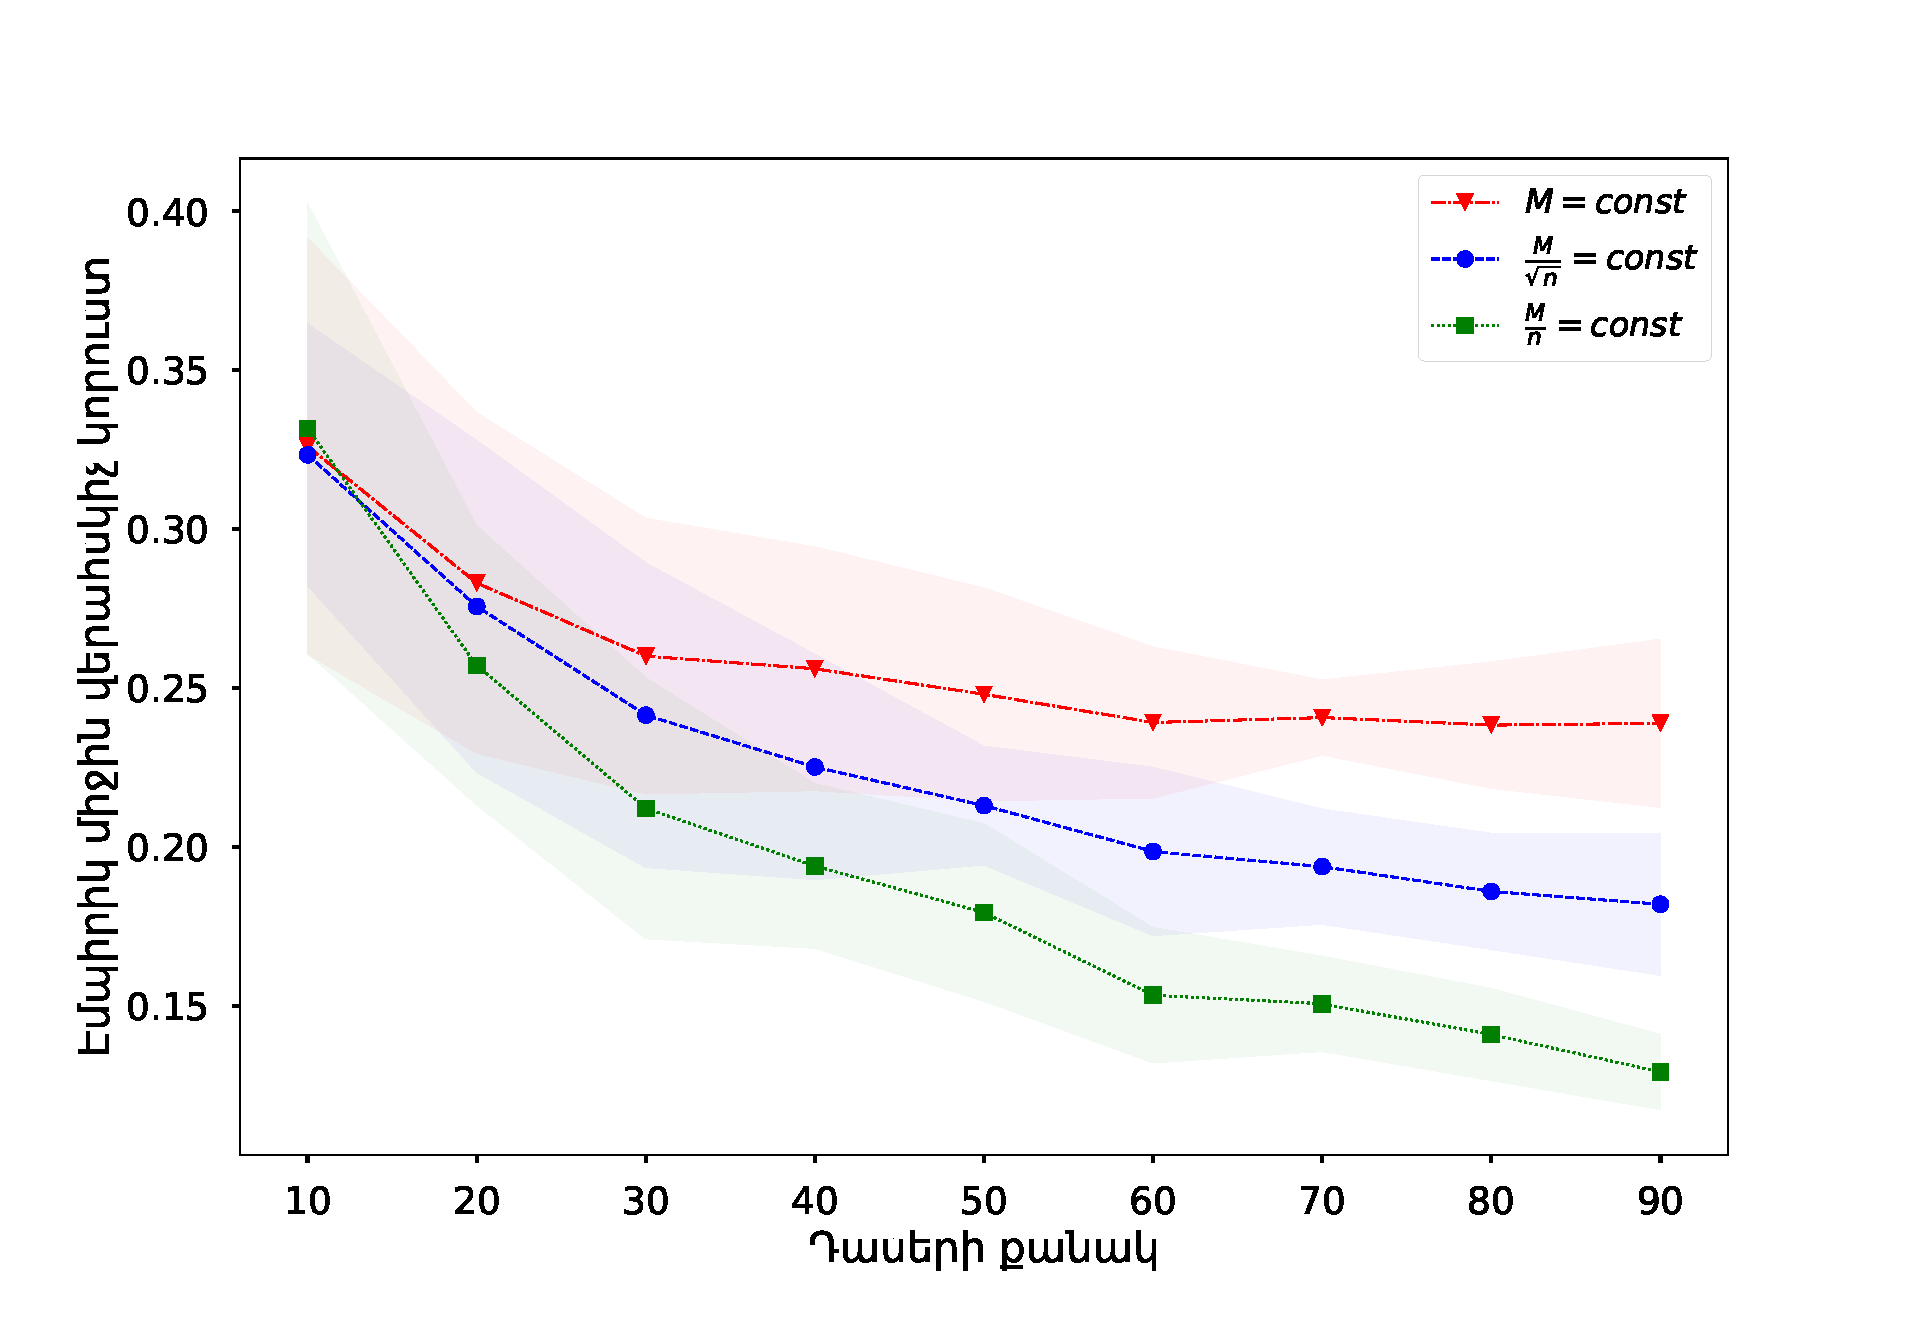
\includegraphics[width=0.8\textwidth]{imgs/k=2.pdf}
\end{figure}
\begin{center}
 \fontsize{7pt}{7pt} 
\armfont \textit{$k=2$ քանակությամբ դասերից բաղկացած առաջադրանքի էմպիրիկ միջին վերահսկիչ կորստի կախվածությունը՝ ներկայացումների ցանցի վարժեցման ժամանակ  օգտագործված դասերի քանակից։}
\end{center}
\end{frame}

\begin{frame}
\begin{figure}[htp]
\centering
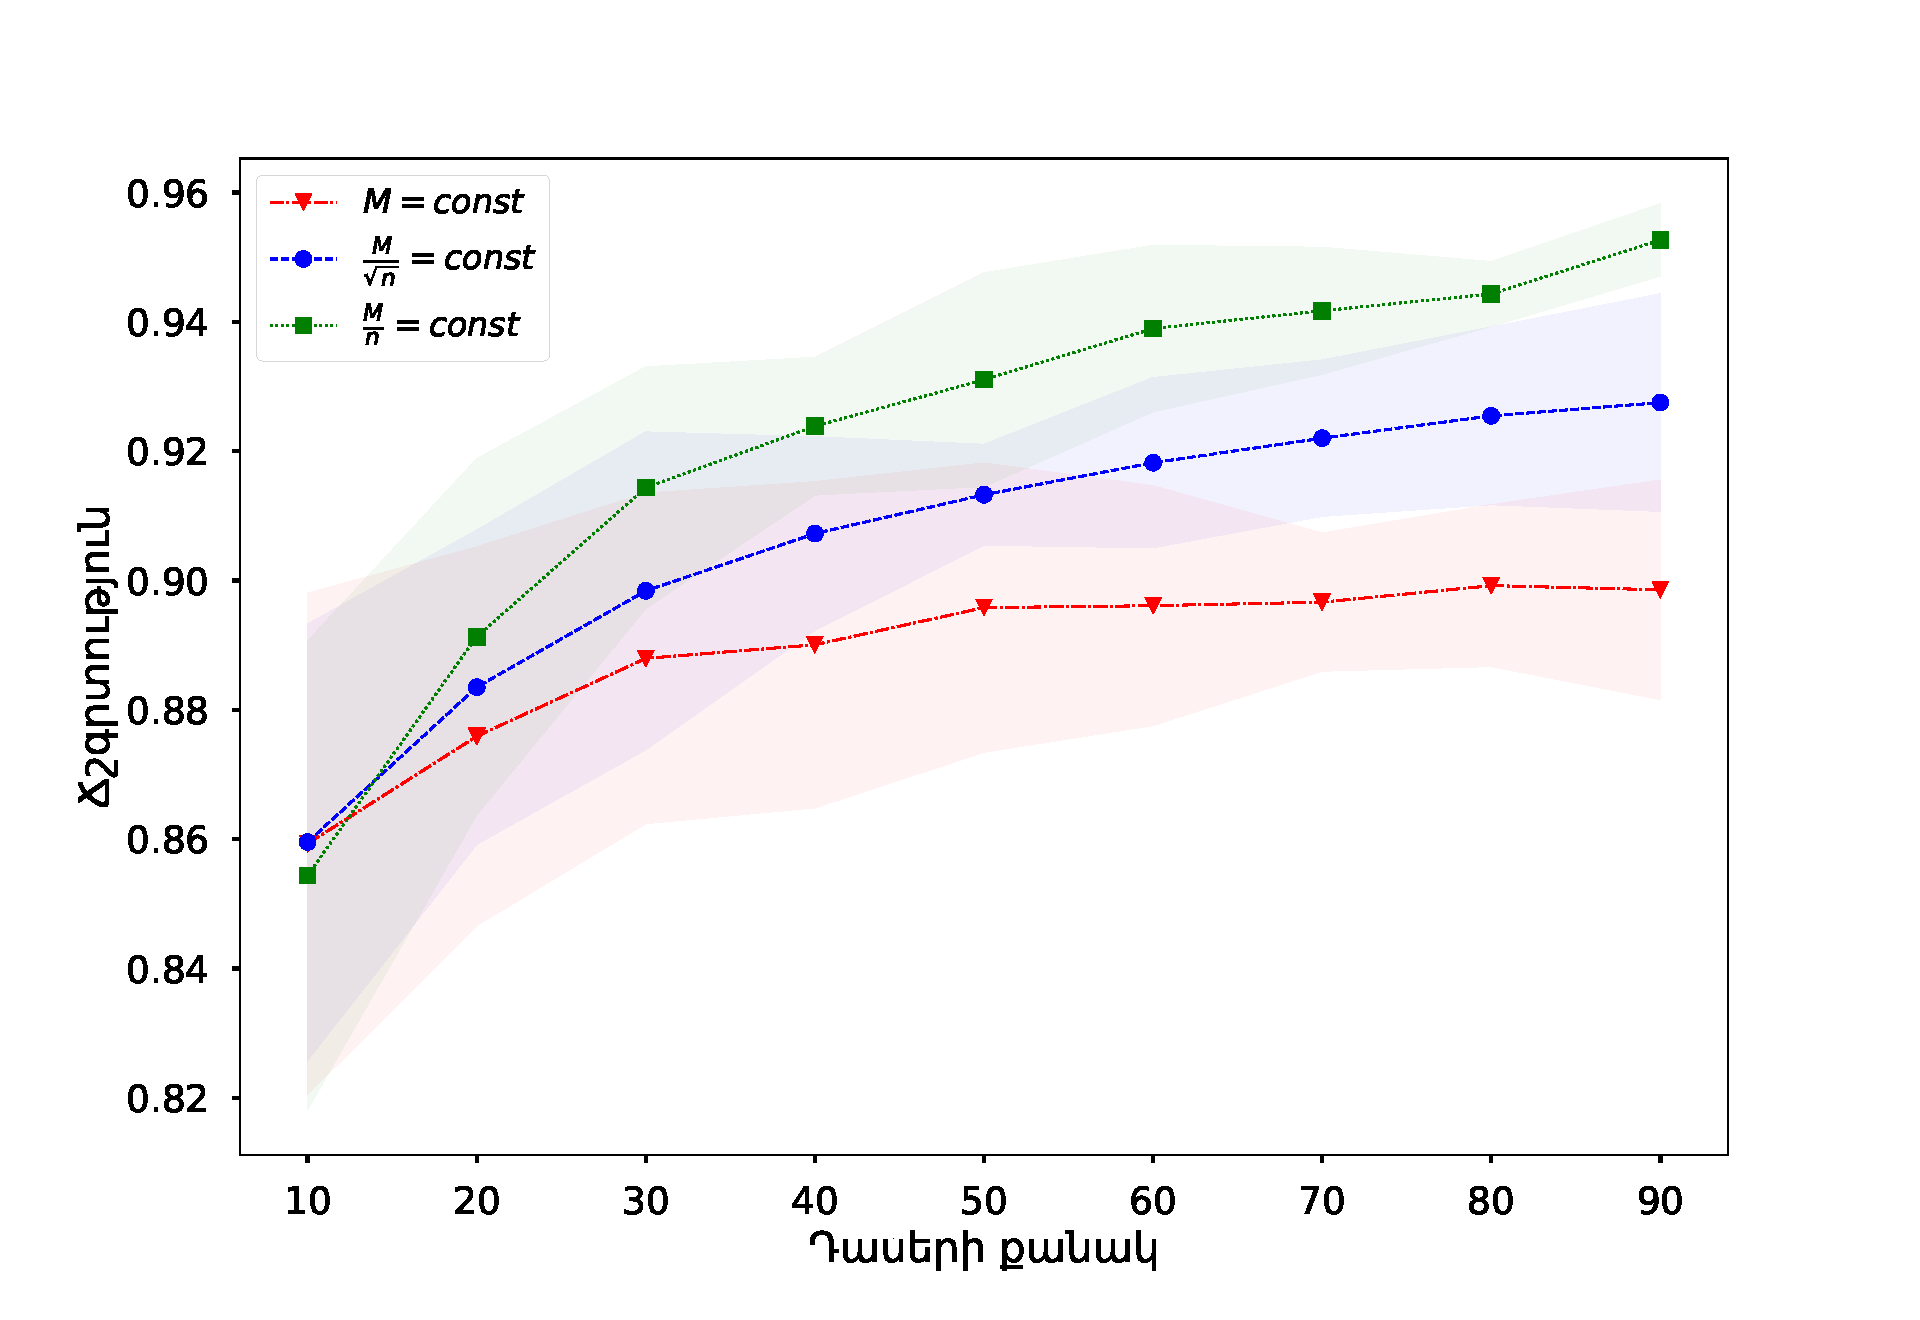
\includegraphics[width=0.8\textwidth]{imgs/k=2_acc.pdf}
\end{figure}
\begin{center}
 \fontsize{7pt}{7pt} 
\armfont \textit{$k=2$ քանակությամբ դասերից բաղկացած առաջադրանքի ճշգրտության կախվածությունը՝ ներկայացումների ցանցի վարժեցման ժամանակ  օգտագործված դասերի քանակից։}
\end{center}
\end{frame}

\begin{frame}
\begin{figure}[htp]
\centering
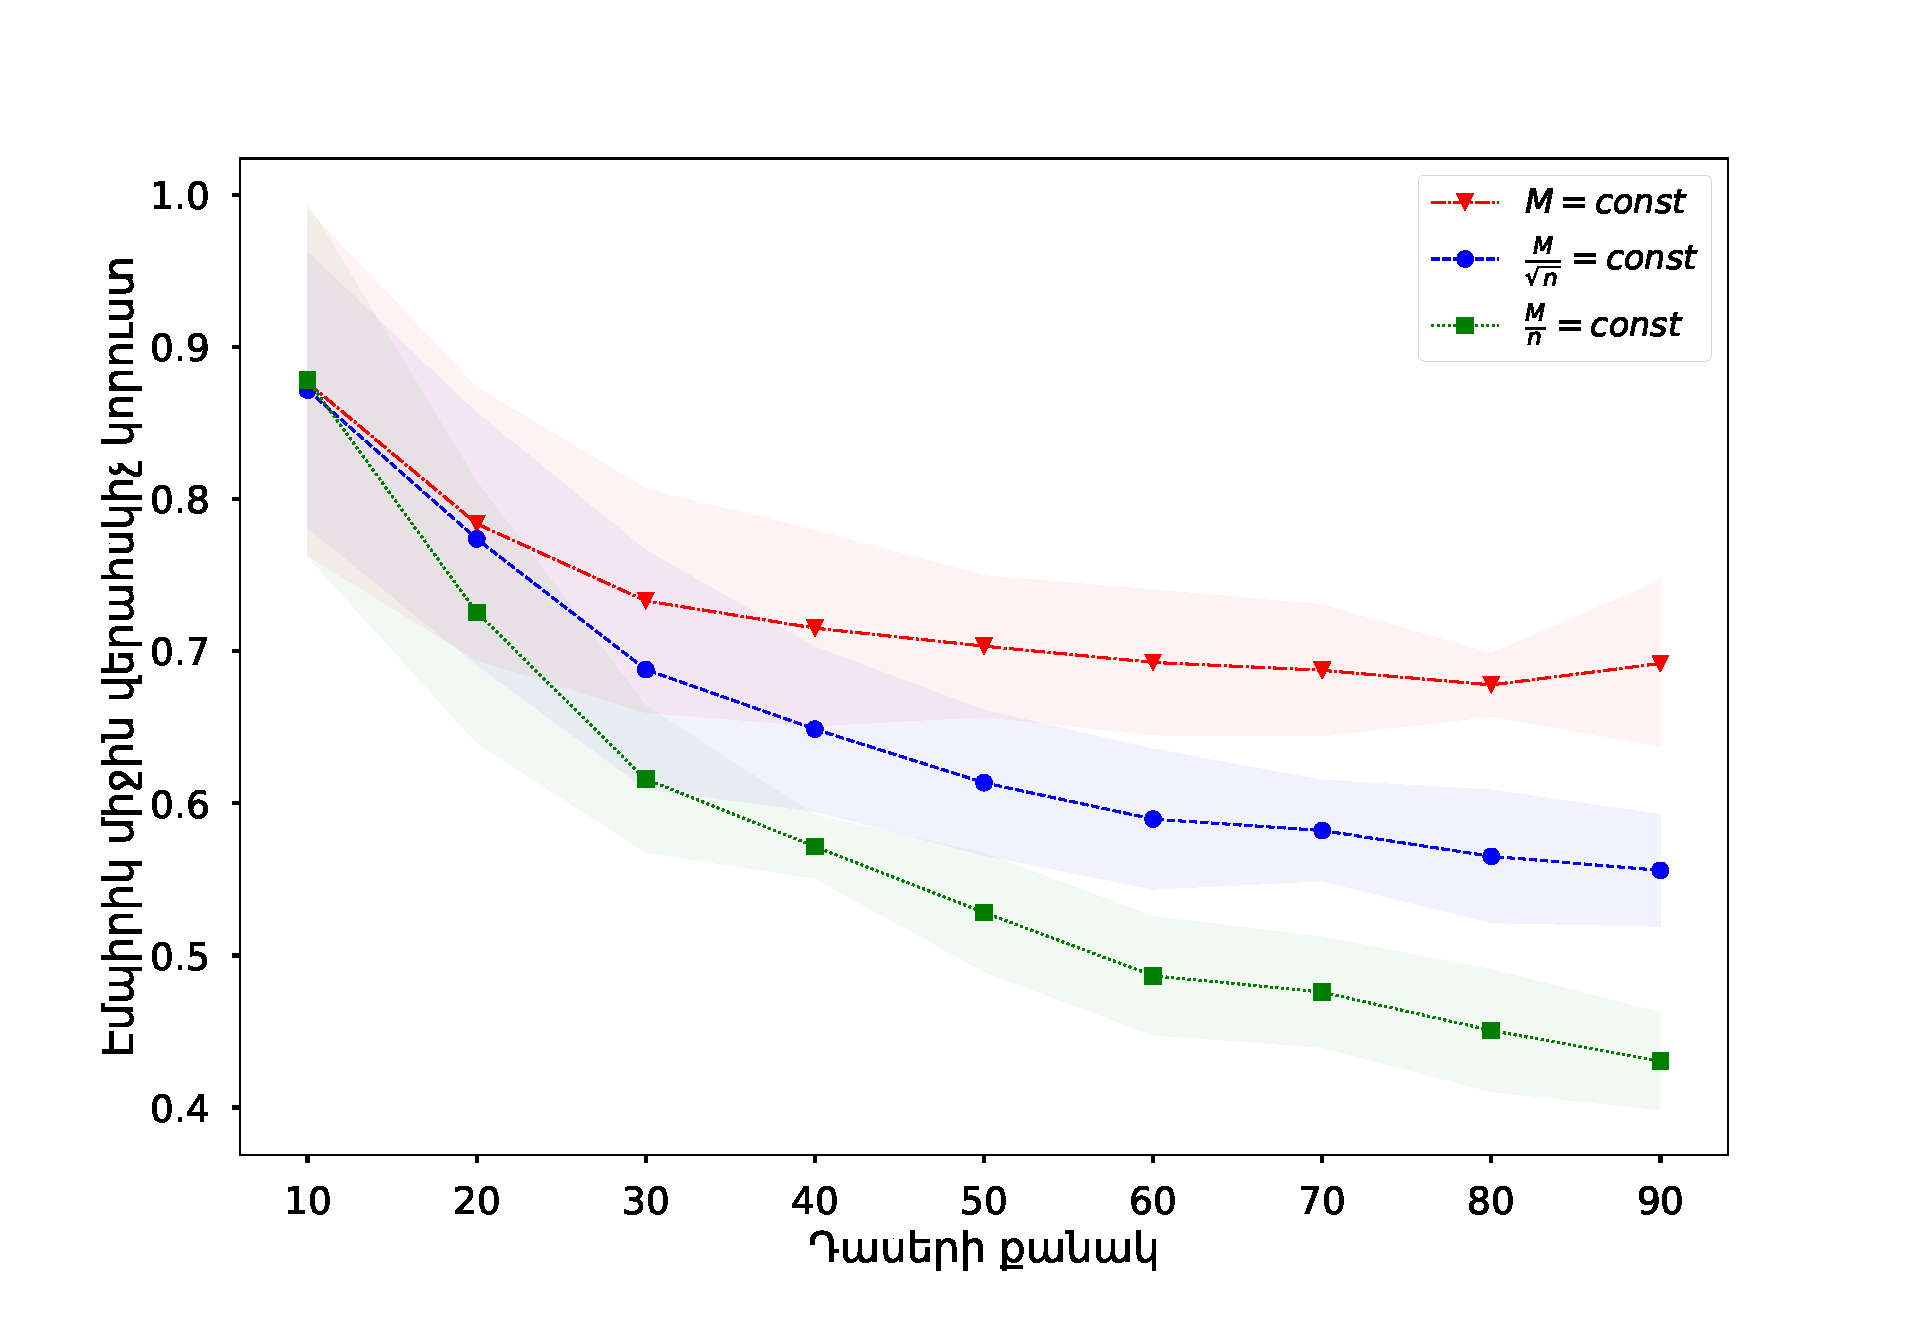
\includegraphics[width=0.8\textwidth]{imgs/k=5.pdf}
\end{figure}
\begin{center}
 \fontsize{7pt}{7pt} 
\armfont \textit{$k=5$ քանակությամբ դասերից բաղկացած առաջադրանքի էմպիրիկ միջին վերահսկիչ կորստի կախվածությունը՝ ներկայացումների ցանցի վարժեցման ժամանակ  օգտագործված դասերի քանակից։}
\end{center}
\end{frame}


\begin{frame}
\begin{figure}[htp]
\centering
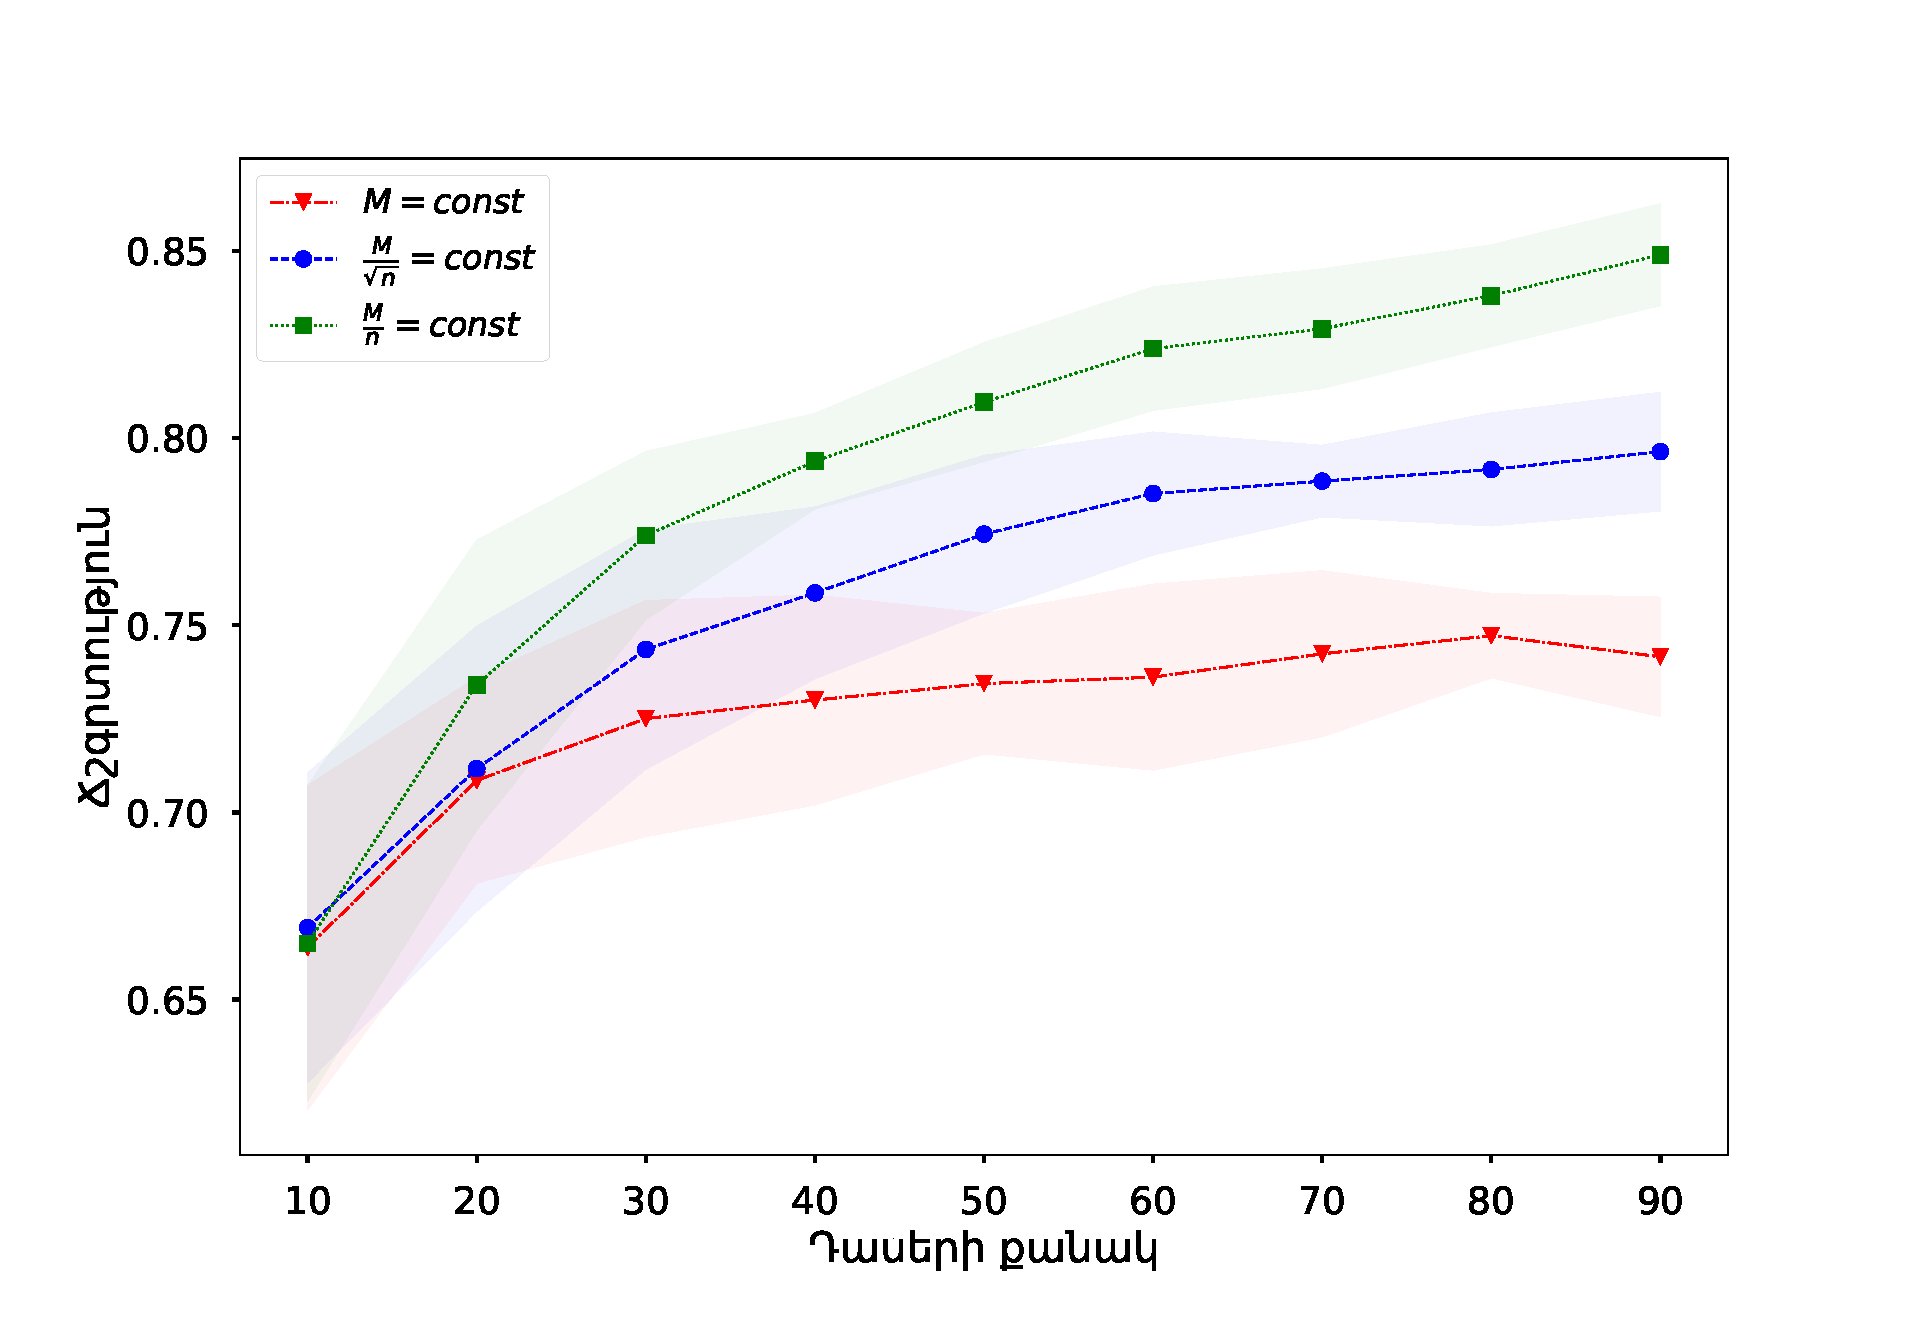
\includegraphics[width=0.8\textwidth]{imgs/k=5_acc.pdf}
\end{figure}
\begin{center}
 \fontsize{7pt}{7pt} 
\armfont \textit{$k=5$ քանակությամբ դասերից բաղկացած առաջադրանքի ճշգրտության կախվածությունը՝ ներկայացումների ցանցի վարժեցման ժամանակ  օգտագործված դասերի քանակից։}
\end{center}
\end{frame}

\begin{frame}
\begin{figure}[htp]
\centering
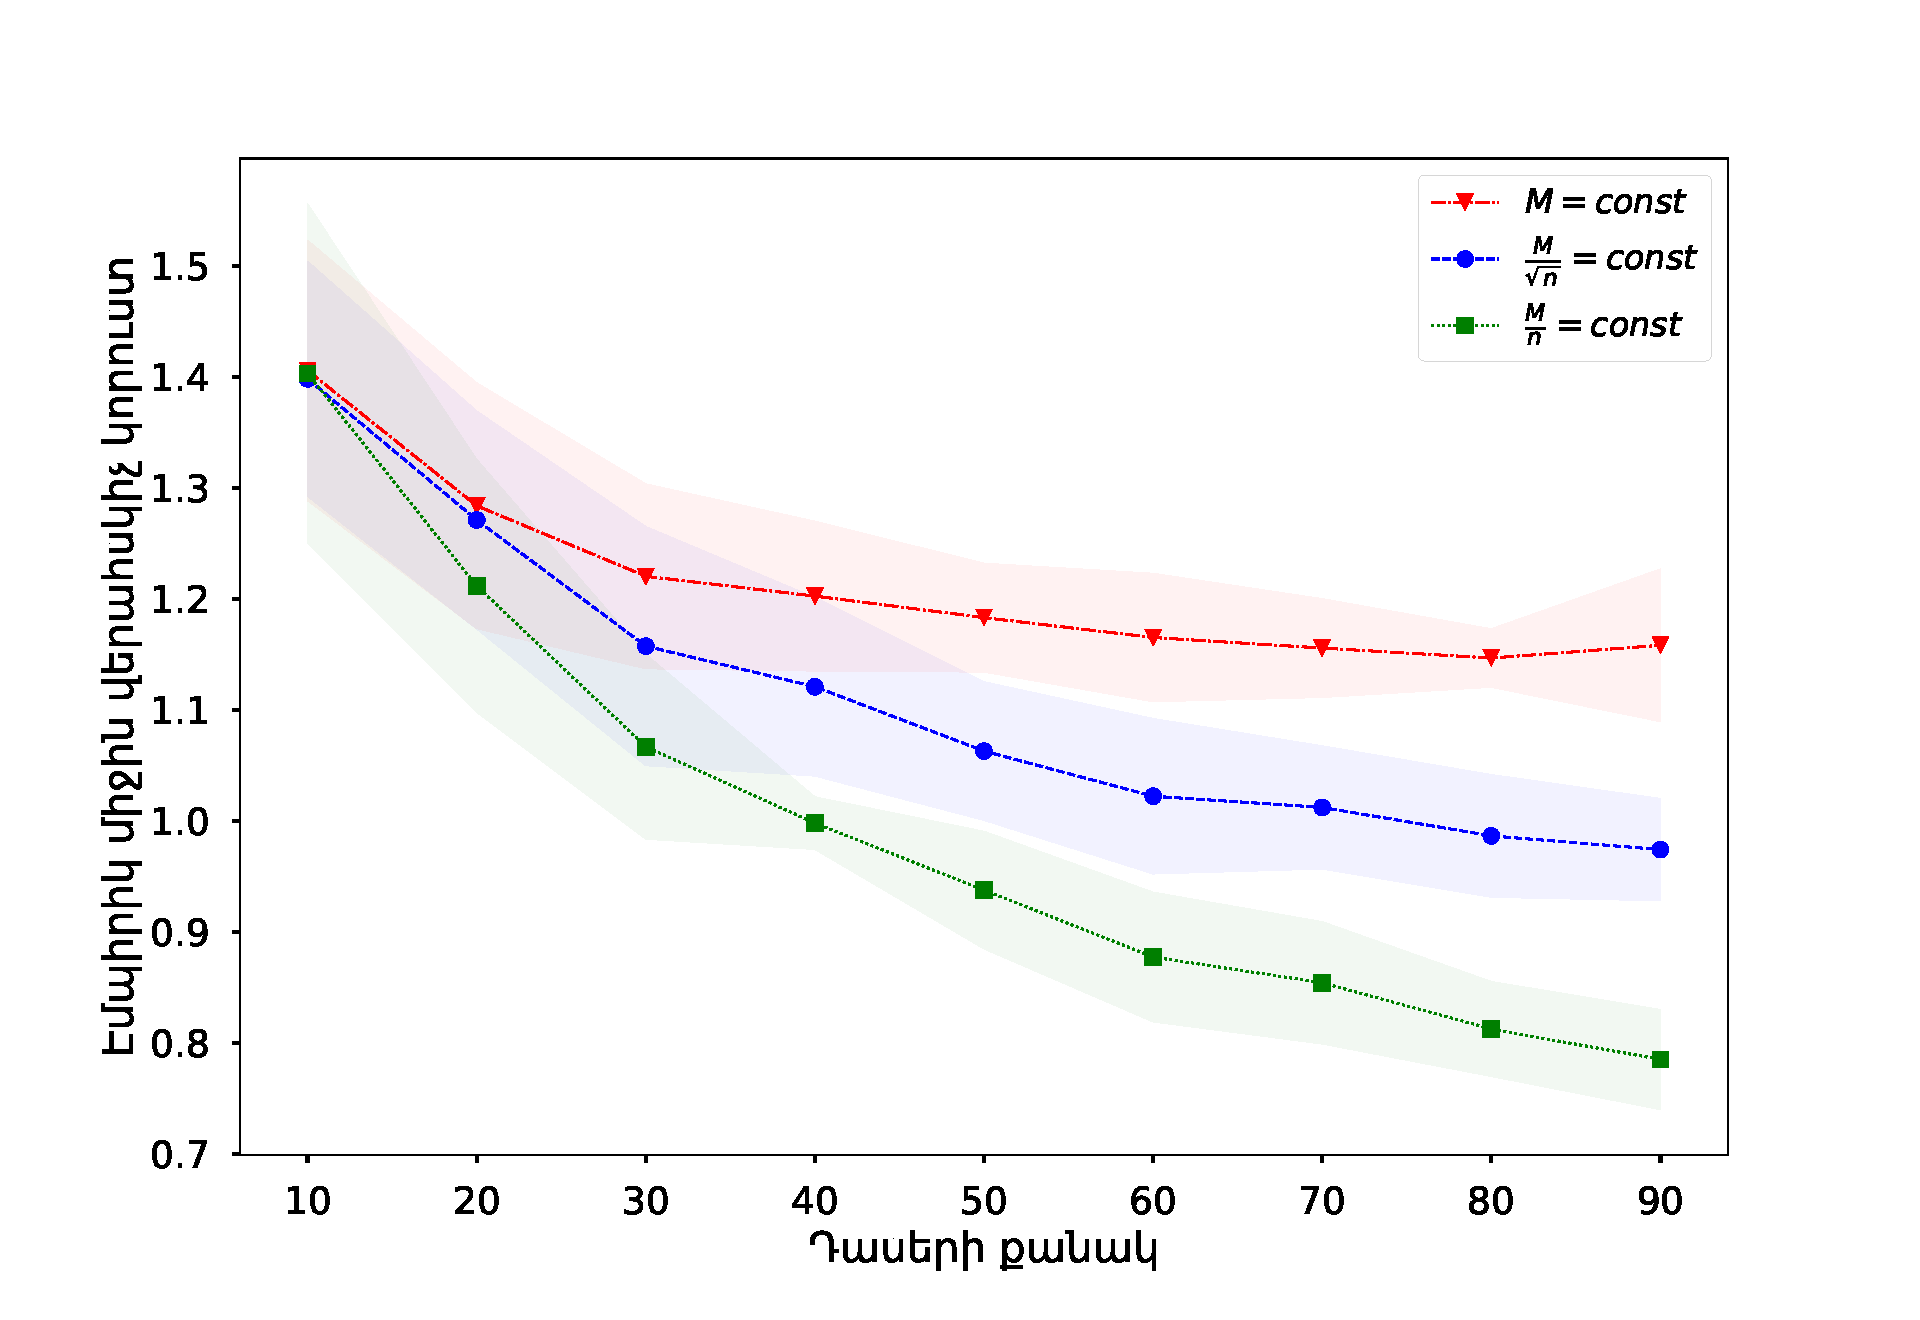
\includegraphics[width=0.8\textwidth]{imgs/k=10.pdf}
\end{figure}
\begin{center}
 \fontsize{7pt}{7pt} 
\armfont \textit{$k=10$ քանակությամբ դասերից բաղկացած առաջադրանքի էմպիրիկ միջին վերահսկիչ կորստի կախվածությունը՝ ներկայացումների ցանցի վարժեցման ժամանակ  օգտագործված դասերի քանակից։}
\end{center}
\end{frame}


\begin{frame}
\begin{figure}[htp]
\centering
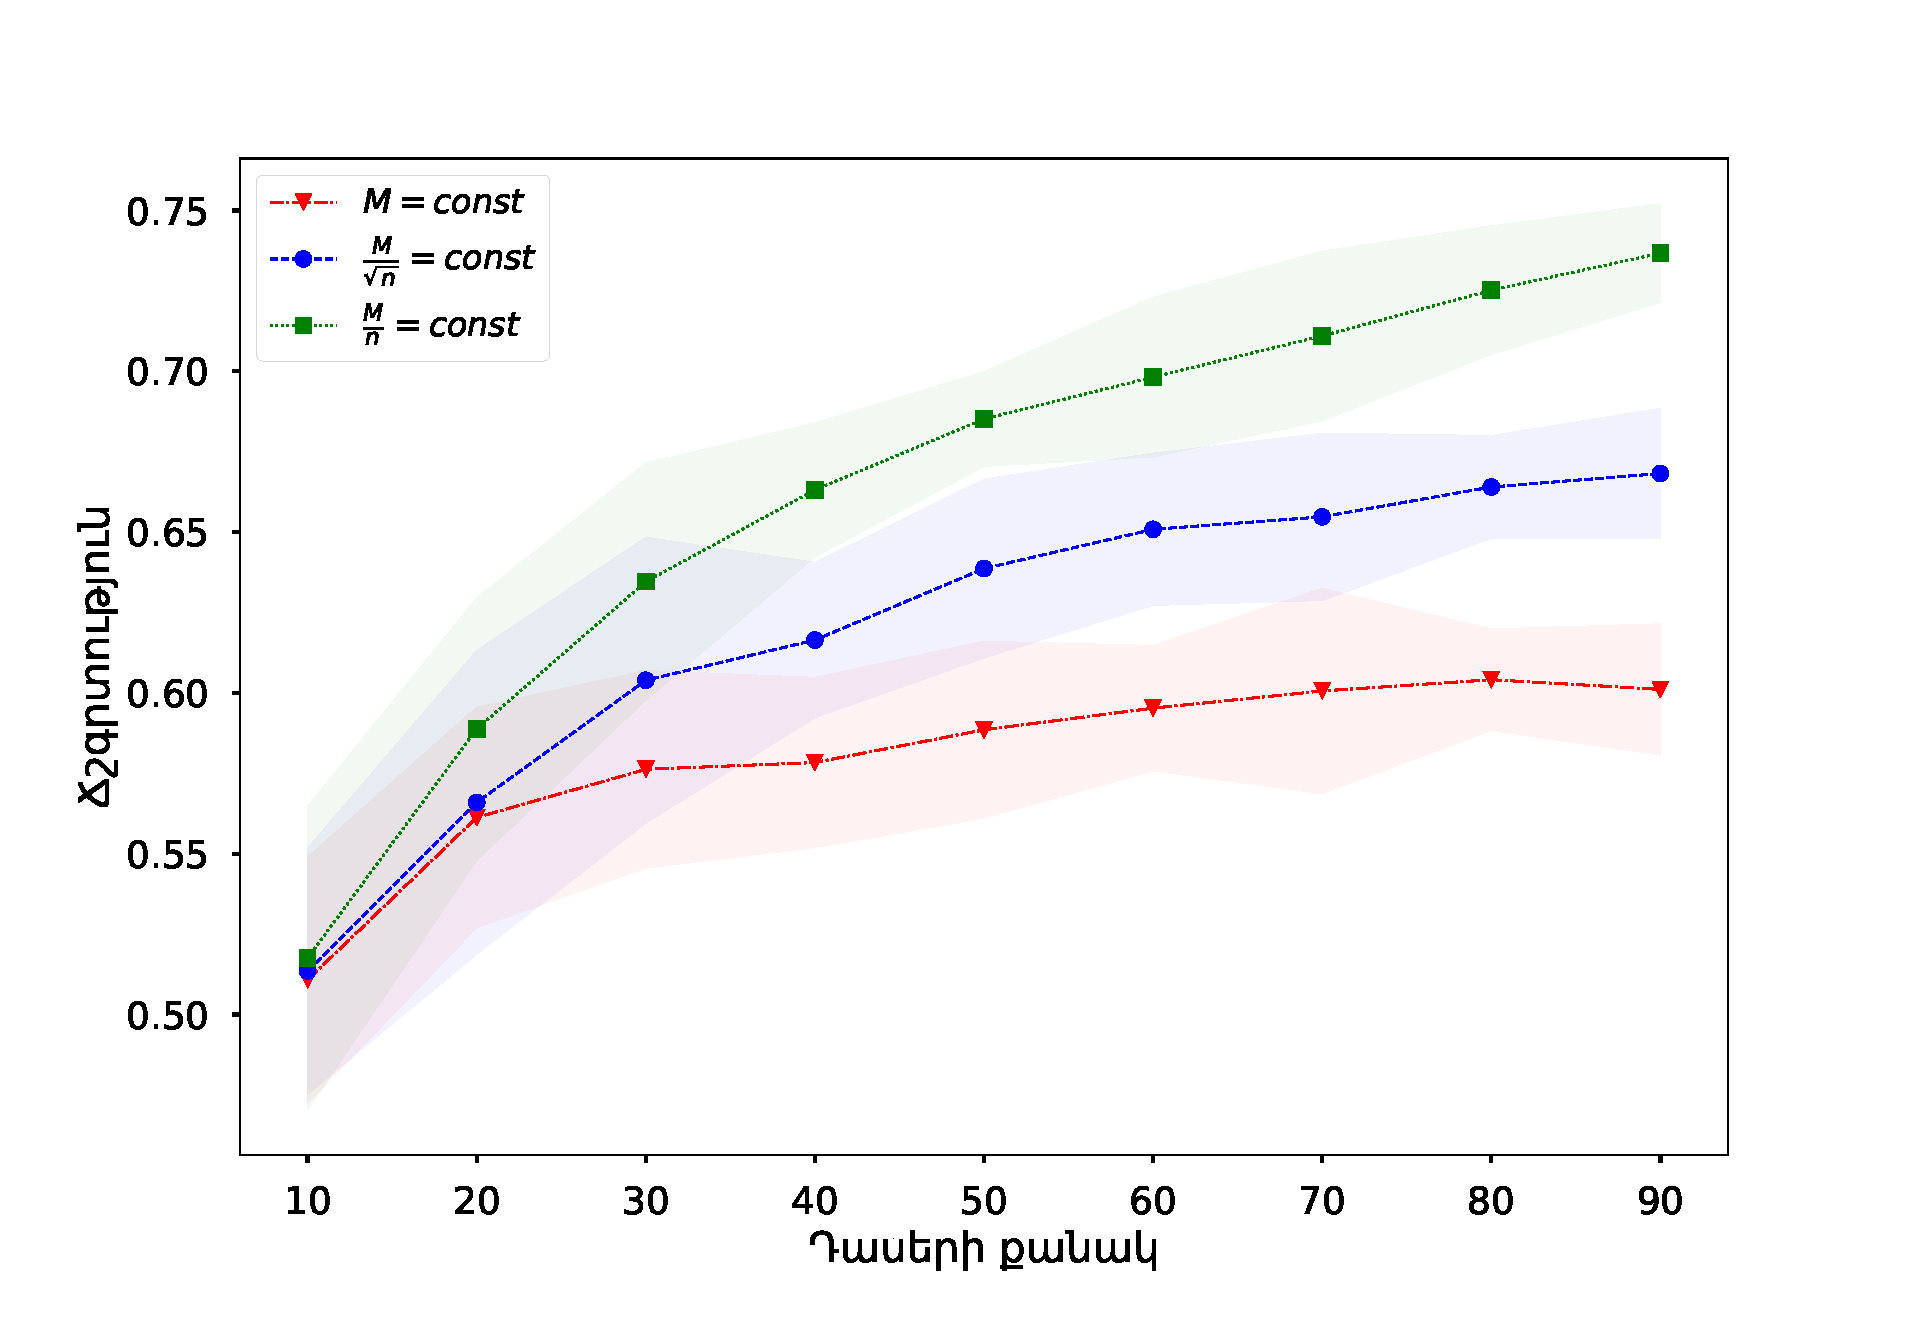
\includegraphics[width=0.8\textwidth]{imgs/k=10_acc.pdf}
\end{figure}
\begin{center}
 \fontsize{7pt}{7pt} 
\armfont \textit{$k=10$ քանակությամբ դասերից բաղկացած առաջադրանքի ճշգրտության կախվածությունը՝ ներկայացումների ցանցի վարժեցման ժամանակ  օգտագործված դասերի քանակից։}
\end{center}
\end{frame}

\begin{frame}
\Wider[4em]{
\begin{center}
 \fontsize{6pt}{6pt} 
\begin{tabular}{|l||r|r|r||r|r|r||r|r|r||}
 \cline{2-10}
  \multicolumn{1}{c|}{} & \multicolumn{3}{|l||}{\hspace{10mm} $M=const$} & \multicolumn{3}{|l||}{\hspace{10mm} $\frac{M}{\sqrt{n}} = const$ } & \multicolumn{3}{|l||}{$\hspace{10mm} \frac{M}{n} = const$} \\
 \cline{2-10}
  \multicolumn{1}{c|}{} &     $k=2$ &     $k=5$ &     $k=10$ &    $k=2$ &     $k=5$ &     $k=10$ &    $k=2$ &     $k=5$ &     $k=10$ \\
\hline
$n=10$                  & $85.930$ & $66.386$ & $51.077$ & $85.955$ & $66.918$ & $51.352$ & $85.440$ & $66.498$ & $51.760$ \\
\hline
$n=20$                 & $87.590$ & $70.856$ & $56.126$ & $88.350$ & $71.168$ & $56.594$ & $89.130$ & $73.404$ & $58.875$ \\
\hline
$n=30$                 & $88.795$ & $72.506$ & $57.624$ & $89.840$ & $74.356$ & $60.393$ & $91.435$ & $77.400$ & $63.458$ \\
\hline
$n=40$                 & $89.005$ & $73.002$ & $57.835$ & $90.725$ & $75.866$ & $61.643$ & $92.385$ & $79.386$ & $66.309$ \\
\hline
$n=50$                 & $89.580$ & $73.442$ & $58.853$ & $91.325$ & $77.436$ & $63.865$ & $93.105$ & $80.966$ & $68.515$ \\
\hline
$n=60$                 & $89.610$ & $73.614$ & $59.526$ & $91.820$ & $78.522$ & $65.085$ & $93.895$ & $82.396$ & $69.817$ \\
\hline
$n=70$                 & $89.665$ & $74.238$ & $60.060$ & $92.200$ & $78.854$ & $65.473$ & $94.170$ & $82.928$ & $71.096$ \\
\hline
$n=80$                 & $89.920$ & $74.724$ & $60.410$ & $92.545$ & $79.166$ & $66.401$ & $94.430$ & $83.810$ & $72.518$ \\
\hline
$n=90$                 & $89.855$ & $74.156$ & $60.107$ & $92.750$ & $79.642$ & $66.821$ & $95.265$ & $84.906$ & $73.671$ \\
\hline
\end{tabular}
\end{center}
}
\end{frame}

\begin{frame}
\armfont
Իրակացված փորձարկումների ծրագիրը հասանելի է հետևյալ հասցեով՝ \url{https://github.com/Gevorg-Minasyan/fine-tune-tj}։
\end{frame}

\iffalse

\begin{frame}[fragile] % Need to use the fragile option when verbatim is used in the slide
\frametitle{Verbatim}
\begin{example}[Theorem Slide Code]
\begin{verbatim}
\begin{frame}
\frametitle{Theorem}
\begin{theorem}[Mass--energy equivalence]
$E = mc^2$
\end{theorem}
\end{frame}\end{verbatim}
\end{example}
\end{frame}

\begin{frame}
\frametitle{Multiple Columns}
\begin{columns}[c] % The "c" option specifies centered vertical alignment while the "t" option is used for top vertical alignment

\column{.45\textwidth} % Left column and width
\textbf{Heading}
\begin{enumerate}
\item Statement
\item Explanation
\item Example
\end{enumerate}

\column{.5\textwidth} % Right column and width
Lorem ipsum dolor sit amet, consectetur adipiscing elit. Integer lectus nisl, ultricies in feugiat rutrum, porttitor sit amet augue. Aliquam ut tortor mauris. Sed volutpat ante purus, quis accumsan dolor.

\end{columns}
\end{frame}

\begin{frame}
\frametitle{Table}
\begin{table}
\begin{tabular}{l l l}
\toprule
\textbf{Treatments} & \textbf{Response 1} & \textbf{Response 2}\\
\midrule
Treatment 1 & 0.0003262 & 0.562 \\
Treatment 2 & 0.0015681 & 0.910 \\
Treatment 3 & 0.0009271 & 0.296 \\
\bottomrule
\end{tabular}
\caption{Table caption}
\end{table}
\end{frame}

%------------------------------------------------

\begin{frame}
\frametitle{Theorem}
\begin{theorem}[Mass--energy equivalence]
$E = mc^2$
\end{theorem}
\end{frame}

%------------------------------------------------

\begin{frame}[fragile] % Need to use the fragile option when verbatim is used in the slide
\frametitle{Verbatim}
\begin{example}[Theorem Slide Code]
\begin{verbatim}
\begin{frame}
\frametitle{Theorem}
\begin{theorem}[Mass--energy equivalence]
$E = mc^2$
\end{theorem}
\end{frame}\end{verbatim}
\end{example}
\end{frame}

%------------------------------------------------

\begin{frame}
\frametitle{Figure}
Uncomment the code on this slide to include your own image from the same directory as the template .TeX file.
%\begin{figure}
%\includegraphics[width=0.8\linewidth]{test}
%\end{figure}
\end{frame}

%------------------------------------------------

\begin{frame}[fragile] % Need to use the fragile option when verbatim is used in the slide
\frametitle{Citation}
An example of the \verb|\cite| command to cite within the presentation:\\~

This statement requires citation \cite{p1}.
\end{frame}

%------------------------------------------------

\begin{frame}
\frametitle{References}
\footnotesize{
\begin{thebibliography}{99} % Beamer does not support BibTeX so references must be inserted manually as below
\bibitem[Smith, 2012]{p1} John Smith (2012)
\newblock Title of the publication
\newblock \emph{Journal Name} 12(3), 45 -- 678.
\end{thebibliography}
}
\end{frame}
\fi
%------------------------------------------------


\begin{frame}
\Huge{\centerline{\armfont{Շնորհակալություն}}}
\end{frame}

%----------------------------------------------------------------------------------------

\end{document} 